\PassOptionsToPackage{american}{babel}
\documentclass[twoside]{article}
\usepackage[american]{babel}
\usepackage[backend=biber,style=apa,sortcites=true,sorting=nyt]{biblatex}
\DeclareLanguageMapping{american}{american-apa}
\addbibresource{./Transenvironmental.bib}
\usepackage{capt-of}
\usepackage{longtable}
\usepackage{setspace}
\usepackage{etoolbox}
\AtBeginEnvironment{longtable}{\singlespacing}
\usepackage{fancyhdr}
\fancyhead[LE,RO]{Mainstreaming Pipeline}
\fancyhead[LO,RE]{Michael Ryan Hunsaker, PhD}
\pagestyle{fancy}
\usepackage{booktabs}
\usepackage{float}
\usepackage{afterpage}
\usepackage{caption}
\usepackage{blindtext}
\usepackage{tabularx}
\usepackage{graphicx}
\graphicspath{ {images/} }
\usepackage[toc,page]{appendix}
\usepackage{pdfpages}
\usepackage{csquotes}
\usepackage{setspace}
\usepackage{geometry}
\usepackage{xcolor}
\usepackage{bookman} 
\usepackage{endnotes}
\usepackage{url}
\usepackage{lscape}
\usepackage{authblk}
\pagenumbering{gobble}
\DeclareCaptionLabelFormat{adja-page}{\hrulefill\\#1 #2 \emph{(previous page)}}
\DeclareCaptionFont{tiny}{\tiny}
%
\makeatletter
\AtBeginEnvironment{tabular}{%
  \def\baselinestretch{1}\@currsize}%
\makeatother
%
\title{Development and Implementation of a Mainstreaming Process to Transition Students from Self-Contained Special Education into General Education Placements}
%\shorttitle{Mainstreaming Pipeline}
%
\author[1]{Michael Ryan Hunsaker, Ph.D.}
\affil[1]{University of Utah, Salt Lake City, UT, USA}
%

%
%\rightheader{Mainstreaming Pipeline}
%\leftheader{Michael Ryan Hunsaker, Ph.D.}
%
\begin{document}
%
\maketitle
%
\begin{abstract}
One challenge presented to special educators is transitioning students out of special education self-contained settings and into the general education classroom. This challenge is compounded by there being an abundance of quality data that to guide placement into the special education classroom, but relatively sparse data exist to support transition out of special education back into the general education population. There are even fewer data demonstrating effective transitions of students out of self-contained classroom environments. To support special educators in these transitions, I developed a set of tools specifically to guide qualified students back into general education. These tools include a \textit{Mainstreaming Decision Tree} to identify candidate students and elucidate successful placement in general education. Identified candidate students then enter a 7-step transenvironmental programming process called a \textit{Mainstreaming Pipeline} to guide them through the process of being selected as a candidate, selection of general education classroom, data collection, and finally how to make the final transition out of special education self-contained placements. In the 2015-2016 school year, I undertook a limited implementation of these transenvironmental programming tools and facilitated the transition of 10 of 20 identified candidate students from self-contained academic special education classrooms into general education placements. In the 2016-2017 school year this pilot implementation was extended to include 4 schools. Sixteen (16) of 53 identified candidate students from self-contained academic special education classrooms were able to transition into general education placements. In an extension of the model district-wide, 9 of 26 identified students from behavior/SEL unit classrooms, and 9 of 9 identified students from Life Skills/SID unit classrooms were successfully transitioned into a general education with part-time special education placement. A high percentage of the remaining candidates received \textgreater50\% of their day in general education classrooms and/or were placed in less restrictive self-contained classrooms. Overall, 54\% of identified candidate students were able to access a less restrictive environment as defined by IDEIA
\end{abstract}
%
\section{Introduction}
It is critical that evidence based transenvironmental programming methods be developed to facilitate the transition of students from self-contained special education classrooms into less restrictive environments present in the cascading services model of special education services. The cascading services model works thus: The most restrictive educational environments are specialized schools, followed by self-contained specialized classrooms, self-contained resource, general education with part-time special education/resource, and with general education without special education services being the least restrictive classroom environment. 

The Individuals with Disabilities Education Improvement Act (IDEIA; \textit{20 USC §1400 et seq Part D, Subpart 3, Sec 682}) states (emphasis mine):
\begin{quote}
(c) Findings. --Congress finds the following:

\qquad (1) Disability is a natural part of the human experience and in no way diminishes the right of individuals to participate in or contribute to society. Improving educational results for children with disabilities is an essential element of our national policy of ensuring equality of opportunity, full participation, independent living, and economic self-sufficiency for individuals with disabilities.

\qquad (2) Before the date of enactment of the Education for All Handicapped Children Act of 1975 (Public Law 94-142), the educational needs of millions of children with disabilities were not being fully met because--

\qquad \qquad (A) the children did not receive appropriate educational services;

\qquad \qquad (B) the children were excluded entirely from the public school system and from being educated with their peers;

\qquad \qquad (C) undiagnosed disabilities prevented the children from having a successful educational experience; or

\qquad \qquad (D) a lack of adequate resources within the public school system forced families to find services outside the public school system.

\qquad (3) Since the enactment and implementation of the Education for All Handicapped Children Act of 1975, this title has been successful in ensuring children with disabilities and the families of such children access to a free appropriate public education and in improving educational results for children with disabilities.

\qquad (4) However, the \textbf{implementation of this title has been impeded by low expectations, and an insufficient focus on applying replicable research on proven methods of teaching and learning for children with disabilities}.

\qquad (5) Almost 30 years of research and experience has demonstrated that the education of children with disabilities can be made more effective by--

\qquad \qquad (A) \textbf{having high expectations for such children and ensuring their access to the general education curriculum in the regular classroom, to the maximum extent possible}, in order to--

\qquad \qquad \qquad (i) meet developmental goals and, to the maximum extent possible, the challenging expectations that have been established for all children; and

\qquad \qquad \qquad (ii) be prepared to lead productive and independent adult lives, to the maximum extent possible;
\end{quote}
%
Special education to general education setting transition pipelines are critical because it is far too often the case that students, once placed in special education, remain in their initial special education placements long after they no longer require those highly specialized and individualized special education services to achieve academic progress \parencite{klotz2005new, johnson2005key, anderson1987consistency, conway1988mainstreaming, fuchs1992case}. Difficulties in moving students back into the general education curriculum has led to suggestions that the cascading or tiered system of special education should be eliminated and replaced with scaffolds in the general education classroom to specifically support students identified with disabilities that impact their educational performance (\textit{cf.}, conservationist vs. abolitionist argument in 1980's and 1990's; \cite{fuchs1994classroom, zigmond1995concluding, anderson1987consistency, conway1988mainstreaming}). 

Lack of mobility toward less restrictive placements within the cascading model of special education is especially problematical for students that were initially placed in special education for behavioral, rather than academic, interventions at a very young age (\textit{e.g.}, Pre-Kindergarten students with autism placed in self-contained classrooms for maladaptive behaviors). The lack of a clear transition process to exit students from full time special education / special class settings can often be detrimental to educational outcomes \parencite{savich2008inclusion}. This is due to the fact that students in special education miss out on access to instructional materials used in the general education classroom and core instruction from highly-qualified grade level teachers \parencite{gersten2006rti,brownell2010special,zigmond1995concluding,fuchs1992case}. 

It has been suggested that special class placements are at best a separate but unequal entity in comparison with mainstream general education classrooms (\cite{skiba2008achieving, bedinim1990separate}; but cf., counterexample in  \cite{kauffman2002separate, mcleskey2012we,}). These arguments have led to discussions regarding IDEIA and the (un)intentional segregation of disabled and non-disabled students within the US public school system \parencite{ferri2005tools, nolan2004us, marchese2000putting, mccarthy2012vestiges,}. What this means is that, at least in the academic literature, the impetus to design methods to integrate disabled students into the general education classroom was greater prior to IDEIA (\textit{cf.}, Peabody Re-Integration Project; \cite{fuchs1994classroom, fuchs1993conservative, daniel1997educating}).

To address these challenges, I propose a decision making a flowchart called a \textit{Mainstreaming Decision Tree} to guide student profiling efforts and a specific \textit{Mainstreaming Pipeline} as specialized tools to guide transenvironmental programming with the aim of transitioning students out of self-contained special education classrooms and into the general education classroom. 

The \textit{Mainstreaming Decision Tree} is a useful tool for self-contained special education classroom teachers to identify candidate students that will benefit from a less restrictive classroom environment. The \textit{Mainstreaming Pipeline} formally assists teachers of identified students to transition them into those less restrictive placements. What makes these processes unique is that, unlike the earlier work on transenvironmental programming that focused primarily on transitioning students from the resource classroom into the general education classroom, the present pipelines were designed to transition students in special classroom placements into the general education environment, both with and without the assistance of part time special education/Resource services. 

The manuscript details the development of these tools and implementation of the \textit{Mainstreaming Decision Tree} and \textit{Mainstreaming Pipeline} to guide students out of self-contained special education and into general education placements.

\section{Methods}
\subsection{Development of a Mainstream Decision Tree}
The primary motivation for the development of a \textit{Mainstreaming Decision Tree} is the idea that access to the general education curriculum is legal right of every student, regardless classification and placement as a special education student \parencite{hocutt1996effectiveness,johnson2005key,conway1988mainstreaming}. Although this need is universally accepted, it is often a difficult proposition to transition students out of self-contained special education classrooms and into general education classroom full time. This can be for reasons of teacher or parent bias \parencite{skiba2008achieving,marden2013criteria, smith2006classroom, praisner2003attitudes} or the difficulties in specifically developing a process by which to undertake this type of a difficult transition \parencite{cauley2006developing,fuchs1994classroom, kalaci2007students}.

To explicitly address these challenges, I developed a process whereby the basic decision making steps for student transition are undertaken in an explicitly (and exclusively) data-driven manner. This method is loosely based on the MTSS process if observed from the point of view of moving down, rather than up, the tiers. This approach supplants the current system that requires teachers to use their best judgment in selecting candidate students for mainstreaming \parencite{fuchs1993conservative,fuchs1994classroom,marden2013criteria,mathes1998preparing,wadsworth1999preparing,wadsworth1999preparing,fuchs1994best}. 

The \textit{Mainstreaming Decision Tree} was designed to focus only on data and thus prevent individuals from being asked or required to make judgment calls that may be informed by personal prejudices or biases regarding student potential for behavior and/or academic achievement \parencite{raines2012universal,reynolds2009response}. Such data-driven decisions are important because decisions not explicitly motivated and supported by data are legally indefensible, particularly if one applies the need for school districts to provide an \textit{appropriate} educational benefit rather than a \textit{de minimus} standard as previously acceptable under legal statutes (580 U.S. 15–827, 2017).

To reduce the occurrence of indefensible special education decisions, the \textit{Mainstreaming Decision Tree} depends on data collected during initial and subsequent special education evaluations. This means that the data used for the decision making process are readily available for virtually all students and relatively standardized, at least within individual school districts or Local Education Agency (LEAs). 

Importantly, these data were collected by multiple members of the IEP team and by related service providers, so there was no single person in charge of both collecting the data and making decision on those results. The \textit{Mainstreaming Decision Tree} can be seen in Figure~\ref{fig1} and is available in an easier to use format in Appendix~\ref{Appendix1}.
%
%%%%%%%%%%%%%%%%%%%%%%%%%%%%%%%%%%%%%%%%%%%%
%
% Begin Figure 1
%
%%%%%%%%%%%%%%%%%%%%%%%%%%%%%%%%%%%%%%%%%%%%
%
\begin{figure*}[htp!]
\centering
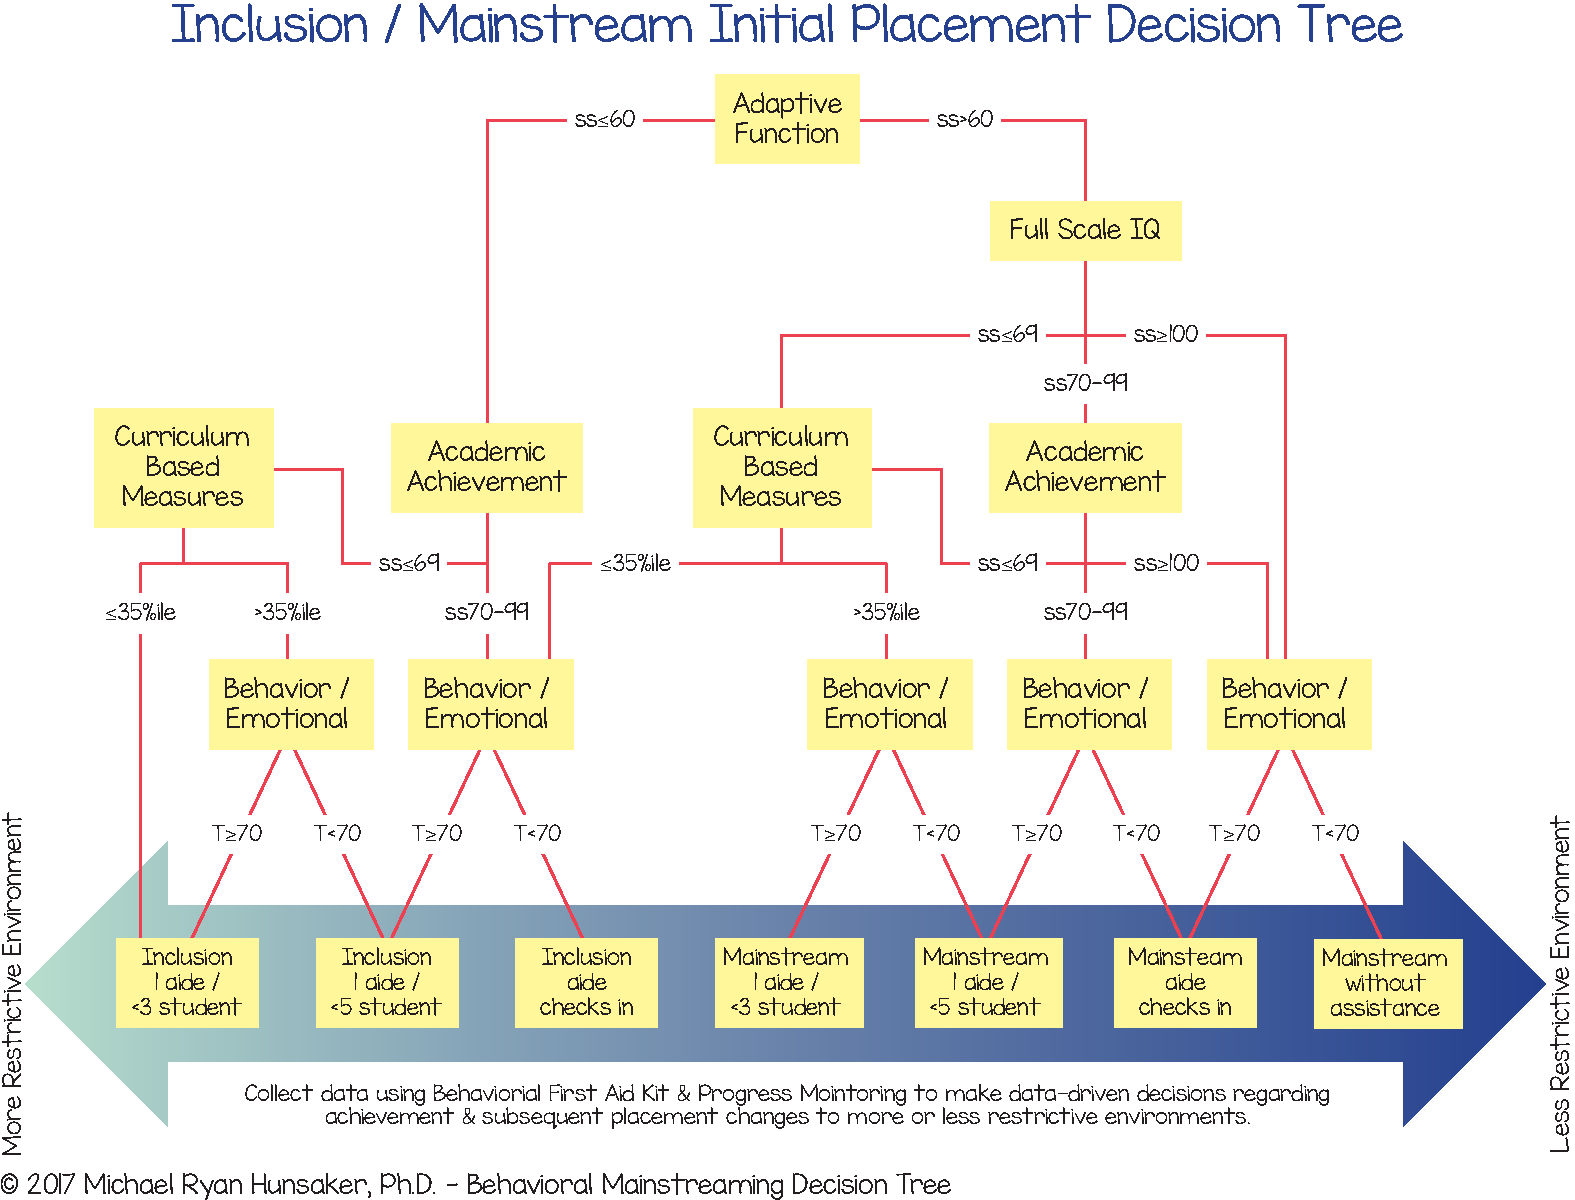
\includegraphics[width=\textwidth]{Figure1.pdf}
\caption[Mainstreaming Decision Tree]{\textit{Mainstreaming Decision Tree. The Mainstreaming Decision Tree is a visual depiction of the data-driven decision making process used to identify candidates for transition from self-contained special education to general education with part time special education/Resource services placements. Data regarding Adaptive Function is the first decision point, followed by Full Scale IQ, Academic Achievement, and Socio-Emotional Well Being. Along the bottom are the spectrum of restrictive environments ranging from inclusion with an aide on the left to independent mainstream access to the general education classroom on the right.}}
\label{fig1}
\end{figure*}
%
%%%%%%%%%%%%%%%%%%%%%%%%%%%%%%%%%%%%%%%%%%%%
%
% End Figure 1
%
%%%%%%%%%%%%%%%%%%%%%%%%%%%%%%%%%%%%%%%%%%%%
%
%%%%%%%%%%%%%%%%%%%%%%%%%%%%%%%%%%%%%%%%%%%%
%
% End of Chapter
%
%%%%%%%%%%%%%%%%%%%%%%%%%%%%%%%%%%%%%%%%%%%%
%
\subsection{Hierarchy of Measures Included in Mainstream Decision Tree}
Table~\ref{tab1} contains all the data types input into the \textit{Mainstream Decision Tree}. Table~\ref{tab2} identifies data types explicitly \textit{excluded} from the decision making process as these are judgment calls that are often primarily informed by personal and professional biases that are indefensible by data. Finally, Table~\ref{tab3} provides research-based cutoff scores that serve to predict student success in the general education classroom.

The hierarchy followed by the \textit{Mainstreaming Decision Tree} is Adaptive Function as the first decision point, followed by Full Scale IQ, Academic Achievement, and finally Socio-Emotional Well Being. These items were placed in this order to maximize predictive validity of the process by emphasizing certain measures at earlier or later stages of decision making. The flow of decision points can be seen in Figure~\ref{fig1} looking from top to bottom.

Important for understanding the intent of the \textit{Mainstreaming Decision Tree} is the operation difference between inclusion and mainstreaming used in this manuscript. The operational definitions used in the \textit{Mainstreaming Decision Tree} and \textit{Mainstreaming Pipeline} are as follows: 
\begin{itemize}
	\item \textit{Inclusion} refers to \textit{social} access to peers in a general education classroom. Assignments are often highly modified for inclusion (assignment modification means entirely different materials or assignments that reduces the expectations on student achievement or alteration to the required curriculum). 
	
	\item \textit{Mainstreaming} refers to \textit{academic} access to the general education classroom. Assignments, tests, and curriculum have to be the same as general education peers or slightly adapted/accommodated (meaning the expectations for achievement and curriculum requirements remain the same, but the assignment can be changed by response mode or reduction of work load to facilitate student success), but cannot be modified. 
\end{itemize}

\subsubsection{Adaptive Function}
Adaptive Function was chosen as the first decision point because of its pivotal role in behavioral flexibility when encountering novel or difficult situations. Adaptive function is an individual's competence of social and practical daily living skills \parencite{de2005adaptive,ditterline2008adaptive,gresham1987relationship}. Adaptive skills are necessary for an individual to adjust their behavior to novel situations or contexts (\textit{i.e.}, change inappropriate behaviors to more appropriate ones given a change to the encountered situation). Adaptive function was emphasized because it underlies the practical, everyday skills needed to function and meet the demands of an individual's environment, including the skills necessary to effectively and independently take care of oneself and interact with other people \parencite{oakland2011adaptive}. Intact adaptive skills are crucial to achieving success in a general education classroom environment. 

Having adaptive function as the first decision point makes the \textit{Mainstreaming Decision Tree} rather conservative so far as taking student coping skills and adaptability into account. Low adaptive composite standard scores result in initially placing the student in more restrictive settings with increased behavioral and academic supports. Once the student responds favorably with these supports, the student progresses toward increasingly less restrictive educational settings. An important note is that if the student appears to show a relative adaptive strength in the sub-measures of adaptive function that relate to schoolwork, that relative strength may be taken into account to generate an alternative path down the \textit{Mainstreaming Decision Tree}. 

\subsubsection{Cognitive/Intellectual Abilities}
Intellectual Abilities (Full Scale IQ) were given lower priority relative to adaptive function simply because a low IQ can be unduly influential if included as the first step of a decision making process. Decades of research suggest IQ measures can be poor predictors or correlates of cognitive ability and academic success in developmentally disabled populations that are well represented in special education classrooms (\textit{e.g.}, spina bifida, autism, and 22q11.2DS; \cite{biswas2016cognitive,dennis2009iq,popa2014atypical,nader2014does}). In fact, it has been demonstrated over and over that there is a bias in IQ tests, with many underestimating the cognitive ability more than others (examples for Stanford-Binet V and WISC-III/IV systematically underestimating cognitive abilities in autism \textit{cf.}, \cite{dawson2007,barbeau2013level,courchesne2015autistic,nader2016does}).

IQ tests measure an individual's cognitive faculties of intellect in comparison to others. The results of IQ tests are proxy to the mental agility of a person. Importantly, intelligence does not cause academic achievement, it simply correlates with achievement measures \parencite{konold1997factor,wechsler2008wechsler}; or, in some cases, FSIQ values fail to correlate with an individual's ability to be successful and may actually underestimate intelligence so greatly as to effect placement decisions \parencite{biswas2016cognitive,dennis2009iq,popa2014atypical,nader2014does}.

\subsubsection{Academic Achievement}
Academic Achievement was chosen to be the next decision step. We focus on the Woodcock-Johnson III NU (WJ-IIINU) and Woodcock-Johnson IV (WJ-IV) because it was the primary tool to assess academic achievement in the school district at the time of this writing. However, the use of appropriate curriculum based measures often gives a more complete snapshot of academic achievement by directly measuring academic skills in the classroom \parencite{mathes1998preparing}. Specifically, with the increasing prevalence of grade-wide common formative assessments (CFA) in the general education classroom, these can be even more reliable indicators of success than standardized achievement tests \parencite{dunn2009critical,heritage2007formative,mathes1998preparing}. As such, curriculum based measures were given priority over achievement scores from the WJ-IIINU.

The WJ-IIINU Tests of Achievement were widely used to assess students for learning disabilities and the resulting data were useful for determining if the students qualify for specialized services. The WJ-IIINU Tests of Achievement uses clusters of tests that directly parallel critical learning goals outlined by IDEIA and provide  procedures for determining discrepancies between student potential and achievement. Curriculum based measures used as direct measure for classroom performance relative to peers in general education environment \parencite{edwards2006factorial,taub2004confirmatory,wu2008short}.

\subsubsection{Socio-Emotional Well Being}
Socio-Emotional Well Being is the final decision point in the \textit{Mainstreaming Decision Tree}. This was intended to quantify anxiety and/or emotional self regulation that deleteriously impact classroom performance. Behavioral and conduct problems that require behavioral intervention can be considered as well at this step (\textit{e.g.}, Behavioral Symptoms Index (BSI) on the BASC-2/3 or Conduct Problems on the Connors 3 and/or Achenbach CBCL). These data were included because behavioral and emotional functioning of children and adolescents are often effective measures for predicting student success \parencite{wiesner2013exploratory}. 

Academic problems, along with problems associated with developing and maintaining positive relationships with others, are often the result of underlying behavioral and emotional challenges. These challenges, when identified and addressed sufficiently early, can be corrected before negatively affecting a child or adolescent \parencite{raines2012universal,reid2004meta}.

The decision to place Socio-Emotional Well Being as the final decision step was deliberate. Once the other factors have been accounted for in the decision making process, this step modulates earlier decisions by placing the student in either a slightly more or less restrictive environment based upon their anxiety and/or behavioral profiles. In other words, Socio-Emotional Well Being was used explicitly to provision increased support for the student if needed to prevent student perception of being overwhelmed by the level of challenge in the classroom. The working model used to describe the role of anxiety or behavioral disorders on student success was based on the Yerkes-Dodson inverted U Law (\textit{cf.}, Figure~\ref{fig2}; \cite{yerkes1908relation,cohen2011yerkes,cooray2005anxiety}).

\subsubsection{Provisioning Academic Support}
Whether to place the student in a more or less restrictive environment is the result of the \textit{Mainstreaming Decision Tree}. As seen in Figure~\ref{fig1}, the \textit{Mainstreaming Decision Tree} results in candidate placements for inclusion or mainstreaming and suggests a level of restrictive environment that will be appropriate for each student. As students exhibit increased independence, academic and behavioral supports can be gradually faded back, resulting in movement toward a less restrictive environment (\textit{i.e.}, toward full independence in the general education classroom). 

Fading back supports is done in two phases, behavioral and academic-with behavioral scaffolds being released first. For both academics and behavior, the first step is to fade supervision based on least restrictive environment. This means reduced access to inclusion para-educators until the student achieves independence. The next step was to provide specific incentives for continued academic success and behavioral successes. 

If students require greater supports in order to be successful, then more supports and scaffolds can be added, moving the student into more restrictive environments that requires less student independence. To scaffold behavioral success, the first step is to provide incentives to build on achieved successes. Then, if necessary, provide behavioral support in the form of a paraprofessional. These supports can take the form of social skills, emotional, or behavioral interventions. 

To provide academic scaffolds, the first step is to provide incentives for continued academic success. If needed, assignments are adapted (assignments are still never modified). Finally, pull-out or push-in academic services are provided to bridge gaps as needed.
%
%
\subsection{Behavioral Mainstreaming Decision Tree}
In parallel with profiling a student's academic needs using the \textit{Mainstreaming Decision Tree}, it is also necessary to quantify their behavioral needs. To accomplish this, I created a \textit{Behavioral Mainstreaming Decision Tree} (Figure~\ref{fig3} and Appendix~\ref{Appendix2}). This was designed for mainstreaming decisions for students in SocioEmotional Learning/Emotional Disturbance/Behavior unit classrooms. 

Similarly to how the academic \textit{Mainstreaming Decision Tree} relies on data rather than teacher or student judgment, the\textit{Behavioral Mainstream Decision Tree} focuses on behavioral data easily collected by the classroom teacher and validated by other staff as fidelity checks. What the \textit{Behavioral Mainstream Decision Tree} does not do, however, is rely on classroom contract or level systems for inclusion/mainstreaming determination \parencite{Smith1993,iwata1974reward}. This decision was made to mitigate the influence of bias on the part of classroom teachers or paraeducators when marking contracts on mainstreaming decisions (\textit{cf.}, \cite{peacock1991problems,PITS:PITS8}). 

\subsubsection{Seclusionary Time Out/Time Out Booth}
The first component of the \textit{Behavioral Mainstream Decision Tree} is whether the behavior of the student require use of seclusionary time out/Time Out Booths or Physical Restraint (also called Forced Physical Guidance and Manual Restraint in some LEAs). The use of these emergency safety interventions is limited in most areas to instances where the behavior of the student is an \textit{immediate and significant danger} to themselves or others. Only the cases of seclusionary time out was used a an Emergency Safety Intervention were considered for the \textit{Behavioral Mainstream Decision Tree}. All other uses were recorded separately and staff were retrained on use of these interventions. If a student requires the use of these interventions,they require instruction in social skills and socio-emotional self regulation prior to attempting any mainstreaming or social inclusion. 

\subsubsection{Physical Aggression}
The second component of the \textit{Behavioral Mainstreaming Decision Tree} is whether the student engages in Physical Aggression. Importantly, this does not include property destruction. A student destroying property and a student attacking another person are very different things and should not be confounded. Physical Aggression includes punching, kicking, slapping, headbutting, using chairs, pencils, etc as weapons to hit another, spitting on, or biting another person. 

Importantly for this component, I differentiate between a physical aggression even if the student was provoked by another student or teacher in the room and those when the student aggresses without clear provocation. Provocation in this sense includes peers or adults making physical contact with a student or restricting their movement. Similarly, using "fighting words" to escalate a student or specifically trigger them is considered provocation. 

\subsubsection{Inappropriate Vocalizations}
The third decision point is that of inappropriate vocalizations. If a student engages in \textit{pervasive} inappropriate language or vocalizations they  will be considered for a more restrictive mainstreaming placement compared to if they do not. For this decision point, inappropriate vocalizations include very specific things: they include screaming used to back off adults or teachers. They also include using specifically course and vulgar language. For clarity, this means if a student is generally talking about Slenderman or killing or hurting someone that \textit{does not} count as an inappropriate vocalization so long as it is not a \textit{credible} threat. If a student uses words like damn, shit, bitch, bastard, fart, poop, etc. I do not count these, regardless the community standards. If students use words like \textit{fuck}, \textit{shit}, \textit{cunt}, \textit{cock}, sexually accurate descriptions of sex organs, descriptions of rape, etc. I do consider these inappropriate vocalizations. I draw this line where I do as the latter vocalizations do not tend to go away in a new environment. The former do.

\subsubsection{Provisioning Behavioral Support}
Similarly to the Mainstreaming Decision Tree, the next component is to choose the level of support necessary for mainstreaming. Meetings should happen biweekly to determine if a more or less restrictive environment is necessary for student success.  As students exhibit increased independence, academic and behavioral supports can be gradually faded back, resulting in movement toward a less restrictive environment (\textit{i.e.}, toward full independence in the general education classroom). 

Fading back supports is done in two phases, behavioral and academic-with behavioral scaffolds being released first. For both academics and behavior, the first step is to fade supervision based on least restrictive environment. This means reduced access to inclusion para-educators until the student achieves independence. The next step was to provide specific incentives for continued academic success and behavioral successes. 

If students require greater supports in order to be successful, then more supports and scaffolds can be added, moving the student into more restrictive environments that requires less student independence. To scaffold behavioral success, the first step is to provide incentives to build on achieved successes. Then, if necessary, provide behavioral support in the form of a paraprofessional. These supports can take the form of social skills, emotional, or behavioral interventions. 

To provide academic scaffolds, the first step is to provide incentives for continued academic success. If needed, assignments are adapted (assignments are still never modified). Finally, pull-out or push-in academic services are provided to bridge gaps as needed.

Critically, if the two different decision trees (academic and behavioral) result in different levels of restrictive environment, the teams will meet to harmonize the differences between the results and what placement is in the best interest of the students. 
%
%
%%%%%%%%%%%%%%%%%%%%%%%%%%%%%%%%%%%%%%%%%%%%
%
% Begin Figure 2
%
%%%%%%%%%%%%%%%%%%%%%%%%%%%%%%%%%%%%%%%%%%%%
%
\begin{figure*}[htp!]
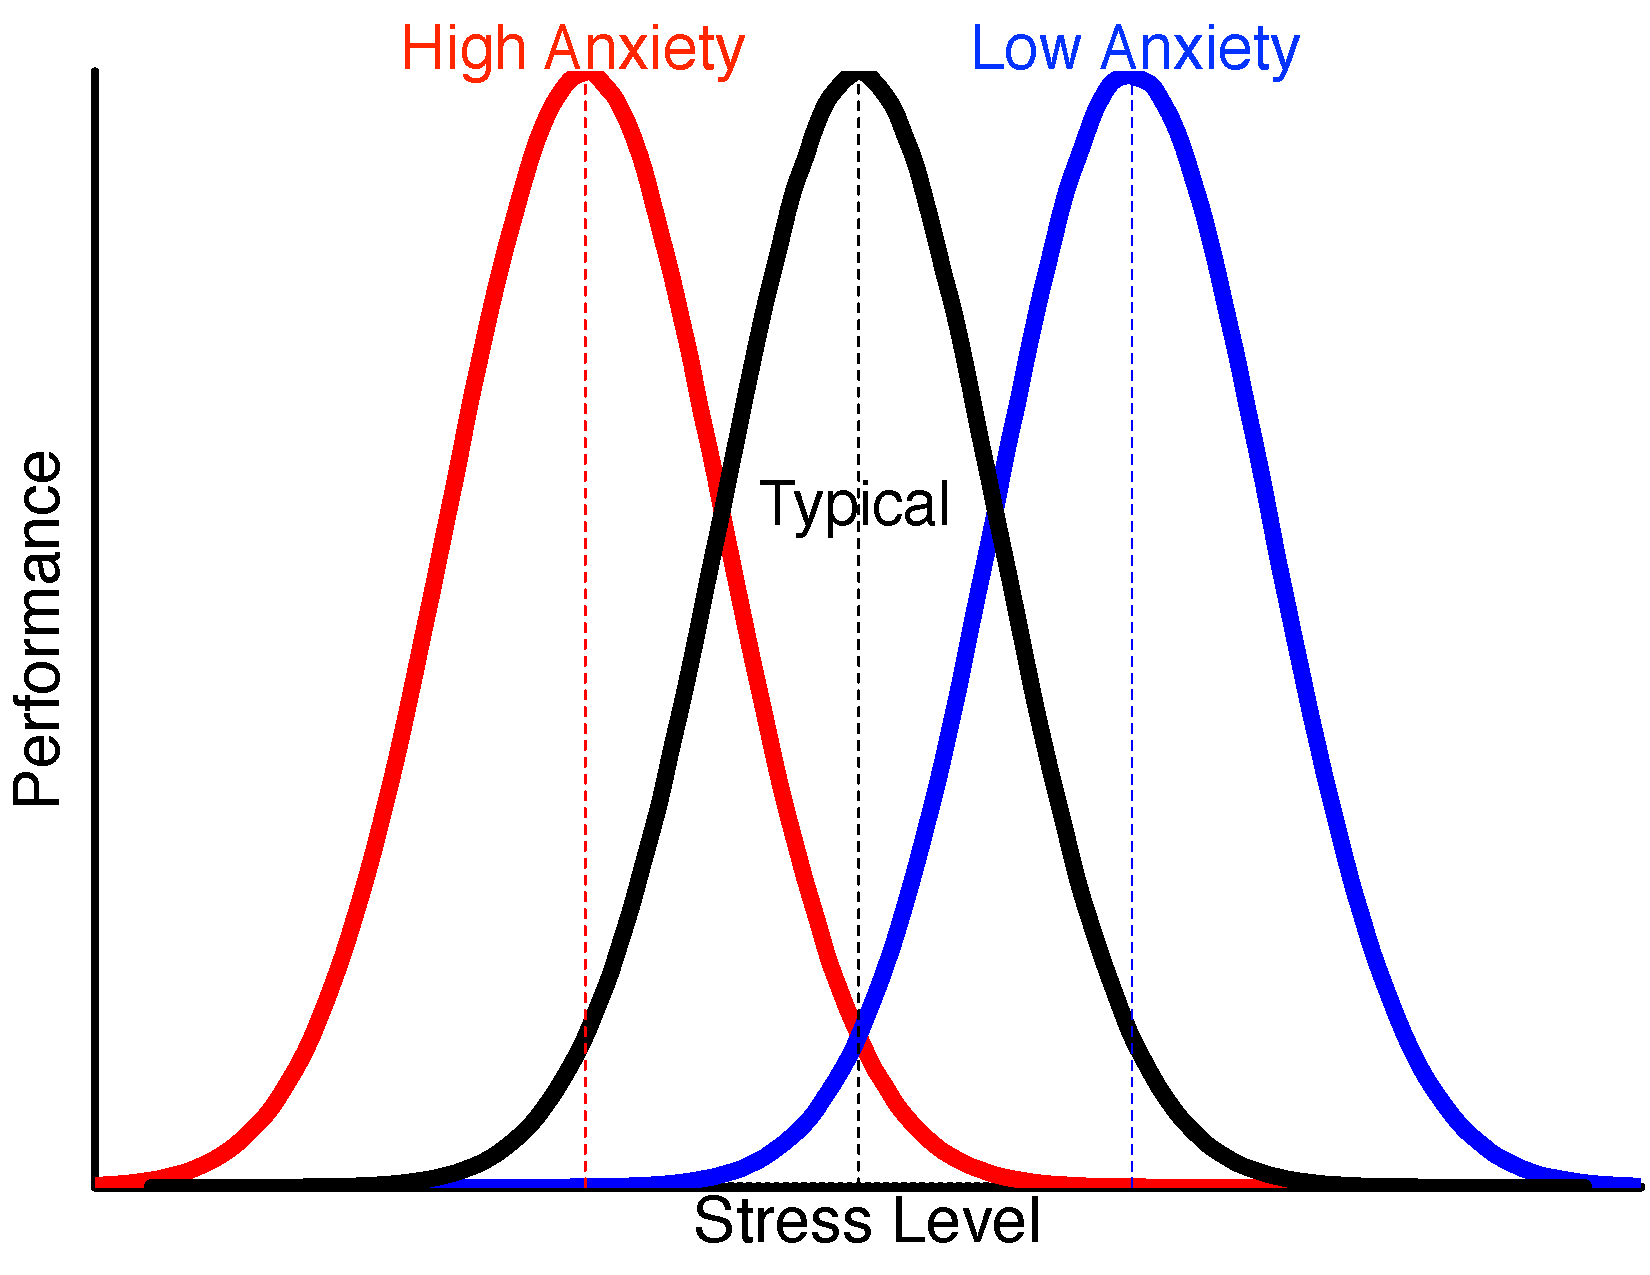
\includegraphics[width=\textwidth]{Yerkes-Dodson.pdf}
\caption[Yerkes Dodson Law]{\textit{Yerkes Dodson Law applied to anxiety after \parencite{yerkes1908relation}. There was a clear relationship between stress and performance, with more stress (or challenge) being required to increase performance up to a point. After that point, there was too much stress and performance decreases. The middle curve line is a model curve for a "typical" student. The high anxiety student line (\textit{e.g.}, T\textsubscript{anxiety}\textgreater70 on BASC 2) shows that student performance peaks at lower stress levels. This suggests the students need increased support to shift the curve rightward where the typical curve is located. Low anxiety student performance peaks at higher stress levels. This suggests they need to be pushed and challenged to shift the curve leftward to where the black curve was located, as they are showing poor performance at "typical" levels of perceived stress.}}
\label{fig2}
\end{figure*}
%
%%%%%%%%%%%%%%%%%%%%%%%%%%%%%%%%%%%%%%%%%%%%
%
% End Figure 2
%
%%%%%%%%%%%%%%%%%%%%%%%%%%%%%%%%%%%%%%%%%%%%
%
%
%%%%%%%%%%%%%%%%%%%%%%%%%%%%%%%%%%%%%%%%%%%%
%
% Begin Table 1
%
%%%%%%%%%%%%%%%%%%%%%%%%%%%%%%%%%%%%%%%%%%%%
%
\begin{table}[tbp]
\centering
\vspace*{0cm}\caption{Data Considered by a Mainstream Decision Tree}
\label{tab1}
\resizebox{\textwidth}{!}
{\begin{tabular}{ccccc}
\hline\\[-1.5ex]
Adaptive & Intelligence & \multicolumn{2}{c}{Academic Achievement} & Emotional \\[0.5ex]
\cmidrule(lr){3-4}
 & & Woodcock Johnson IIINU/IV & Curriculum Based Measurements & \\
\hline\\[-1.5ex]
VABS 2/3 & Stanford Binet V & Reading Skills & District Benchmarks & BASC 2/3\\
ABAS 2/3 & Weschler Nonverbal (WNV) & Reading Comprehension & Utah Compose & Connor's 3\\
BASC 2/3 (Adaptive) & WISC III/IV/V & Math Calculation & AIMS Web & Achenbach CBCL\\
 & Woodcock Johnson IIINU/IV & Math Reasoning & DRA 2 & \\
 & KBIT 2 & Broad Writing (includes Spelling) & Spelling City & \\
 & Leiter R & Broad Reading & GoMath Benchmark, Chapter Tests & \\
 & UNIT 2 & Broad Math & Eureka Math &\\
 & DAS & & DIBLES Next &\\
 & Batelle & & Success Maker &\\
 & & & Imagine Learning &\\
 & & & Reflex Math &\\
 & & & Common Formative Assessments (CFA) &\\
 & & & \textbf{Any evidence-based measure approved by IEP team} &\\
\hline
\end{tabular}}
\end{table}
%
%%%%%%%%%%%%%%%%%%%%%%%%%%%%%%%%%%%%%%%%%%%%
%
% End Table 1
%
%%%%%%%%%%%%%%%%%%%%%%%%%%%%%%%%%%%%%%%%%%%%
%
%%%%%%%%%%%%%%%%%%%%%%%%%%%%%%%%%%%%%%%%%%%%
%
% Begin Table 2
%
%%%%%%%%%%%%%%%%%%%%%%%%%%%%%%%%%%%%%%%%%%%%
%
\begin{table}[tbp]
\centering
\caption{Data \textit{Not Considered} by a Mainstream Decision Tree}
\label{tab2}
\begin{tabular}{l}
\hline\\
Behavioral data from the self-contained classroom\\
Past lack of success in mainstreaming\\
Past lack of school skills necessary for mainstreaming\\
Anecdotal reports of any kind not supported by data\\
Requirement for para-educator time or increased classroom resources\\
Student idiosyncrasies/peculiarities\\
Student personality\\
Parent concerns about academic abilities\\
Parent concerns about behavioral abilities\\
Social skills deficits\\
Student mobility issues\\
\quad Requirement for Orientation \& Mobility Services \\
\quad Use of assistive technology \\
Special education classification\\
Information regarding disability severity\\
Student speech issues\\
\quad Selective Mutism \\
\quad Aphasia \\
\quad Apraxia \\
\quad Stuttering \\
\quad Prosody Errors \\
Medical/Psychiatric diagnoses\\
\quad Autism\\
\quad ADHD\\
\quad Epilepsy\\
\quad Tic Disorders\\
\quad Tourette's\\
\quad ODD, OCD, Bipolar, BPD, etc.\\
\quad Anxiety/Depression status \\
\quad Sensory Impairments \\
\qquad Visual Impairment/Blindness \\
\qquad Deafblindness \\
\qquad Hearing Impairment/Deafness \\
Current or past medications\\
Medication compliance or noncompliance\\
Hesitation of parents to pursue psychiatric help for student\\
Quality of Relationship Teacher has with Parent\\
"Red Flag" or helicopter parent \\
\hline
\end{tabular}
\end{table}
%
%%%%%%%%%%%%%%%%%%%%%%%%%%%%%%%%%%%%%%%%%%%%
%
% End Table 2
%
%%%%%%%%%%%%%%%%%%%%%%%%%%%%%%%%%%%%%%%%%%%%
%
%
%%%%%%%%%%%%%%%%%%%%%%%%%%%%%%%%%%%%%%%%%%%%
%
% Begin Table 3
%
%%%%%%%%%%%%%%%%%%%%%%%%%%%%%%%%%%%%%%%%%%%%
%
\begin{table}[tbp]
\centering
\caption{Cutoff/Criteria Performance Levels for Mainstream Decision Tree}
\label{tab3}
\begin{tabular}{cc}
\hline \\
Adaptive & Intelligence\\
\hline \\
VABS II/3 or ABAS II/3 & Any FSIQ, NVIQ, or VIQ Measure\\
SS \textless60 & SS \textless70\\
SS \textgreater60 & SS 70-100\\
BASC 2/3 (Adaptive) & SS \textgreater100\\
T \textless30 & \\
T \textgreater30 & \\
\hline \\
Academic & Socio-Emotional\\
\hline \\
WJ-IIINU/IV & BASC 2/3/Connor's 3/CBCL\\
SS \textless70 \& RPI \textless18 & T \textless70\\
SS 70-100 \& RPI 18-34 & T \textgreater70\\
SS \textgreater100 \& RPI \textgreater34 &\\
\hline
\end{tabular}
\end{table}
%
%%%%%%%%%%%%%%%%%%%%%%%%%%%%%%%%%%%%%%%%%%%%
%
% Begin Table 3
%
%%%%%%%%%%%%%%%%%%%%%%%%%%%%%%%%%%%%%%%%%%%%
%
%
%%%%%%%%%%%%%%%%%%%%%%%%%%%%%%%%%%%%%%%%%%%%
%
% End of Chapter
%
%%%%%%%%%%%%%%%%%%%%%%%%%%%%%%%%%%%%%%%%%%%%
%
\subsection{Mainstreaming Pipeline}
Once candidate students were identified and placed in an appropriate setting for inclusion/mainstreaming using the \textit{Mainstreaming Decision Tree}, then a specific transenvironmental programming process needs to put into place to guide students toward success in increasingly less restrictive environments. This pipeline was designed to simultaneously build student confidence and ability by stretching and challenging them both academically and behaviorally while providing sufficient scaffolds and support to prevent student failure. To achieve effective transenvironmental programming methods, we developed a 7-step \textit{Mainstreaming Pipeline} based on previous research \parencite{fuchs1993conservative,fuchs1994classroom,marden2013criteria,mathes1998preparing,wadsworth1999preparing,wadsworth1999preparing}. 

\subsubsection{Step 1 - Identify Candidate Students}
As described above, candidate students were identified with the \textit{Mainstreaming Decision Tree} using broad Adaptive scores (Adaptive Composite Standard Score from ABAS-II/ABAS-3 or VABS-II/VABS-3 or else adaptive T-score on BASC2/3), Full Scale IQ (or NVIQ/VIQ as appropriate), Academic Achievement (CBM/CFA or WJ-IIINU/IV), and Socio-Emotional Well Being. To do this, a copy of the \textit{Mainstreaming Decision Tree} was printed off and a highlighter was used to trace down the decision points for each student individually to identify initial inclusion/mainstreaming placement options. The values at each decision point were annotated in a Mainstreaming Data Sheet (form available as Appendix~\ref{Appendix2})

Note, not at this point nor at any other point moving forward were special education classification, medical diagnoses, mobility problems, speech issues, or anything else included in Table~\ref{tab2} considered as factors affecting placement decisions. Neither did teachers consider past difficulties in mainstreaming except as motivation for the development of behavioral plans to scaffold student success. The final element within this step was to write a very precise description of each student in terms of temperament and relative need for structure compared to peers (both compared to special education and grade level general education peers).

\subsubsection{Step 2 - Identify Classroom Placements}
Once candidate students are identified, it becomes critical to identify grade level classrooms as placement options. There are two approaches to doing this: First, one can identify teachers with a known history of working with special education. Second, one can refrain from limiting candidate classrooms to any given teacher, but look at all grade level classrooms to determine best placement options on a student by student basis.

The preferred option is to evaluate all grade level classrooms as candidate placements. This prevents issues associated with the special education department overwhelming a relatively small number of teachers with extra students while not impacting other classrooms within the school \parencite{avramidis2000survey,barnes2015teachers, mukherjee2000inclusion}.Additionally, all efforts were made to spread students in the same grade across classrooms rather than grouping them together. This ws done for two reasons. The first being to prevent overloading a general education classroom with multiple potentially burdensome students. The second reason was to foster independence by challenging the special education students in a new environment without being able to use their peers as a crutch for either bad behavior or seeking help instead of persevering during academic tasks.  Any teacher-student personality considerations based on the profile completed in Step 1 should be addressed with the building administrator prior to moving forward with any placements. 

\subsubsection{Step 3 - Classroom Ecological Inventory}
This step involves harmonizing the special education and general education environments to maximize the potential for student success. It was based strongly on the evidence based transenvironmental programming methods employed by the Peabody Reintegration Project and refined by Fuchs and colleagues \parencite{fuchs1993conservative,fuchs1994classroom,marden2013criteria,mathes1998preparing,wadsworth1999preparing,wadsworth1999preparing}. 

The individual steps/components to this Classroom Ecological Inventory process are as follows: 
\begin{enumerate}
\item Special education teacher (or district facilitator/coordinator) observes candidate general education classrooms to identify any issues that will limit success as well as identify classroom factors that will increase probability of student success. 

\item The special education and general education teachers independently complete a shared ecological inventory for their classrooms that can be used to identify any discrepancies in classroom environment that may impact student success (modified after previous examples in the literature \cite{fuchs1994classroom,marden2013criteria}). In other words, the special education and general education teachers describe their classroom environment, expectations, management styles, etc. The form developed in for the \textit{Mainstreaming Pipeline} is available as Appendix~\ref{Appendix4}.

\item Any discrepancies in the teachers' responses to the inventory were identified and discussed to identify and anticipate potential difficulties for the student moving forward.

\item The general education and special education teachers discuss plans/solutions to potential difficulties for the student based on the data from the ecological survey. The most common issues observed were increased rigor of curriculum in general education compared to special education, insufficient student independence, and different curricula between special education and general education. The most commonly proposed solutions were planned accommodation of assignments (to be faded over time), increasing academic rigor in the special education classroom as the student is transitioning to the general education context, and special education classrooms increasing homework load prior to the transitions so the student develops the academic skills required by homework. 

\item The special education and general education teachers specifically plan classroom accommodations for moving forward. This step involves a number of informal meetings and an in depth conversation as to precise expectations regarding student performance in the general education classroom. The district facilitator often had to intervene at this stage to verify that expectations for the special education student were both realistic but also aligned to expectations for the other students in the classroom. 
\end{enumerate}

Critically, it was emphasized that there could be \textit{zero assignment modification} during any step of the mainstreaming process. Assignments could be adapted so the student could access the curriculum (\textit{e.g.}, change response mode or reduce total work load), but no expectations for curriculum or content mastery would be reduced. Such modifications have been shown to impede long term transition out of special education, whereas appropriate accommodations increase the probability of future success and a reduction in the need for future accommodations \parencite{fisher2003special,fuchs2003responsiveness,hollenbeck1998teachers}.

\subsubsection{Step 4 - Initiate Student Placement in General Education Classroom}
The \textit{Mainstreaming Decision Tree} can be used to identify the specific needs of the student for support levels. At this time need for para-educator allocation and student specific behavior plans are discussed (\textit{cf.}, section \textit{Behavioral Mainstreaming Decision Tree} in the next section). The student is placed in the general education classroom for ~50\% time to begin (unless the IEP team decision was to start with a greater percentage of time).

Upon beginning to attend the mainstream classroom, the special education teacher begins data collection on student independence using a Mainstreaming Data Sheet (Appendix~\ref{Appendix2}). Data collection on independence, levels of accommodation necessary for student success, and classroom behavior were also collected by a district facilitator/coordinator. Behavioral data sheets used during this implementation are available as editable digital files by request or available as Appendix~\ref{Appendix5}

\subsubsection{Step 5 - Transition from Part-Time to Full-Time General Education}
Student time is increased in the general education class until they independently participate 90-100\% of the time in the general education classroom and/or Resource classroom \textit{prior to} moving toward a re-evaluation/placement change. Any increases of student time in general education classroom or movement in the direction of transitioning toward change of placement are based on the following factors: 1) Independence as quantified by a Mainstreaming Data Sheet, 2) Classroom observations, 3) Work completion, and 4) Academic progress, primarily referring to how much accommodation the student needs (\textit{i.e.}, whether or not the student completes coursework with the same assignments as peers receiving only part time special education/Resource services). This final criteria is important because the majority of students transitioning out of self-contained classrooms will need part time special education/Resource services to achieve success.

\subsubsection{Step 6 - Formal Transition from Special Education to General Education}
The IEP team performs an official data review to determine how to proceed with a change of placement. Additional academic testing can be administered (\textit{e.g.},WJ-IIINU/IV) as part of a re-evaluation to elucidate present levels of academic functioning and performance if CBM benchmarks and CFA performance were insufficient. These results guide IEP goal development and to ascertain appropriate levels of part time special education/Resource services.

During this transition, the IEP team develops all necessary behavior plans, contracts, trackers, etc. Any plans or contracts must be designed to fit seamlessly into the school PBIS framework or other school-wide discipline system.

\subsubsection{Step 7 - Transition from Unit School to Neighborhood School}
At the end of the year, there should be a transition meeting with the student's neighborhood school to discuss necessary accommodations, successes, challenges, etc. The following issues need to be discussed: 1) Transition plans: decisions need to be made whether the student returns to their neighborhood school or stay at the school wherein they attended the self-contained classroom. 2) Staffing issues across both schools: It is imperative the schools verify that the impact of any given student or group of students transitioning from one environment to another will not overwhelm individual teachers or grade levels the subsequent year. However, staffing at a particular school is insufficient reason to restrain decisions involving moving students back to their neighborhood schools. This was a discussion among the building administrators of the individual schools (not the teachers). Finally, 3) What transitional assistance the next school year by district facilitator/coordinator should look like.

The two school teams need to develop a set of transitional IEP goals to scaffold the student into a new school/grade/placement, preferably with goals geared toward full student independence in the general education classroom. Additionally, there needs to be a conversation regarding how often a district facilitator/coordinator explicitly checks in on transitioned students at their new school.
%
%
%%%%%%%%%%%%%%%%%%%%%%%%%%%%%%%%%%%%%%%%%%%%
%
% Begin Figure 3
%
%%%%%%%%%%%%%%%%%%%%%%%%%%%%%%%%%%%%%%%%%%%%
%
\begin{figure}[htp!]
	\centering
	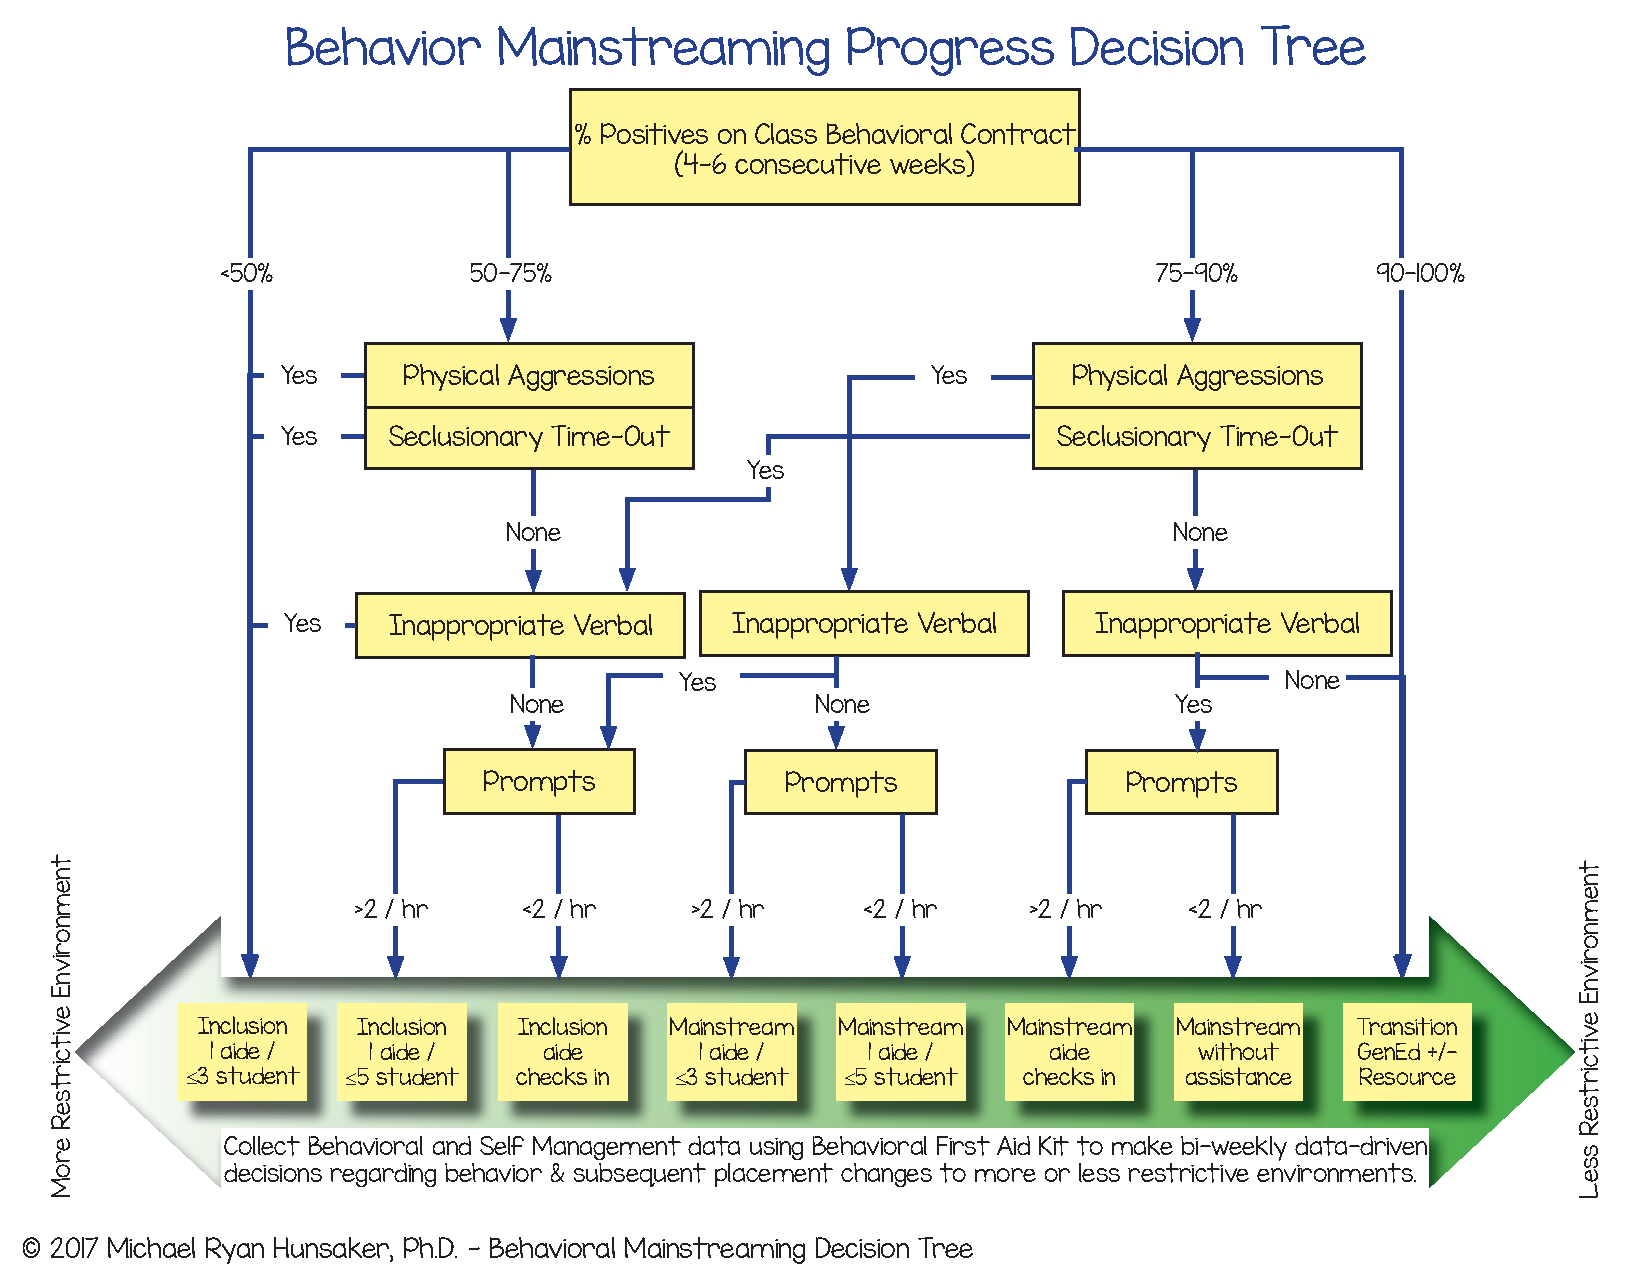
\includegraphics[width=\textwidth]{BehaviorPipeline.pdf}
	\caption[Behaviroal Mainstreaming Decision Tree]{\textit{Behavioral Mainstreaming Decision Tree. The Behavioral Mainstreaming Decision Tree is a visual depiction of the data-driven decision making process used to identify candidates for transition from self-contained special education to general education with part time special education/Resource services placements. Data regarding behavioral performance in self contained and general education classroom are collected and taken into account. Biweekly meetings are held to determine if student needs more or less restrictive environments. Along the bottom are the spectrum of restrictive environments ranging from inclusion with an aide on the left to independent mainstream access to the general education classroom on the right.}}
	\label{fig3}
\end{figure}
%
%%%%%%%%%%%%%%%%%%%%%%%%%%%%%%%%%%%%%%%%%%%%
%
% End Figure 3
%
%%%%%%%%%%%%%%%%%%%%%%%%%%%%%%%%%%%%%%%%%%%%


%%%%%%%%%%%%%%%%%%%%%%%%%%%%%%%%%%%%%%%%%%%%
%
% End of Chapter
%
%%%%%%%%%%%%%%%%%%%%%%%%%%%%%%%%%%%%%%%%%%%%
\section{Results}
\subsection{Results - 2015-2016}
In the first year of this pilot implementation, we identified 20 students (17 male, 3 female - the ratio roughly matched the gender demographics in these special education classrooms) as candidates for transition from the self-contained classroom into a general education with part time special education placement using the \textit{Mainstreaming Decision Tree}. 10 of these students were classified as Autism, 6 as Significant Learning Disabled (SLD), 1 as Speech and Language Impairment (SLI), and 1 as Other Health Impairment (OHI). Students identified as candidates for transition from self contained special education to general education placements ranged from 1\textsuperscript{st} through 5\textsuperscript{th} grade. 6\textsuperscript{th} grade students were not included in this preliminary implementation.

The mean adaptive composite standard score for these 20 students was SS 73.2 +/- 10.37 (standard deviation - SD). The mean full scale IQ standard score was SS 93.3 +/- 10.34 SD. The mean WJ-IIINU academic achievement standard scores were as follows: Reading Skills 86.72 +/- 16.1 SD ; Reading Comprehension 80.21 +/- 15 SD ; Math Calculation 79.1 +/- 24.3 SD; Math Reasoning 78.1 +/- 21 SD; Broad Writing 74.89 +/- 12.92 SD.

Overall, of the 20 students, 5 of the 20 candidate students had anxiety or BSI T scores T \textgreater70 on the BASC, Connor's, or CBCL (25\%). The 20 students that were identified as potential candidates based on these scores from their special education files appeared to be a clear outlying group when compared to their peers across all measures.

Once identified, these students were observed by a single observer (M.R.H.) for two weeks to identify any behavioral issues that could potentially impede access to the general education curriculum. At the same time, students were receiving in-class academic placement examinations to group or classify them into appropriate learning levels within their self-contained classroom. Many of these students were identified as already being able to access (or master) all levels of the special education curriculum at the beginning of the year. All the students in the classroom were also administered district benchmarks and many of the curriculum based measures listed in Table~\ref{tab1}. Based upon success on these measures students were considered candidates for transition out of the self-contained special education classroom.

Profiles of all the students that were candidates for a transition from a self-contained special education classroom to the general education placement are presented in Table~\ref{tab4}.

\subsubsection{5\textsuperscript{th} Grade}
Four 5\textsuperscript{th} grade students successfully transitioned from a self-contained special education placement to a general education with part time special education services placement. One 5\textsuperscript{th} grade student finished the year spending \textgreater75\% time in the general education and the IEP team will consider a transition during the next school year.

\subsubsection{4\textsuperscript{th} Grade}
Two 4\textsuperscript{th} grade students successfully transitioned from a self-contained special education placement to a general education with part time special education services placement. One 4\textsuperscript{th} grade student was unable to access the grade level CBM and was unable to transition into the general education environment. One 4\textsuperscript{th} grade student was unable to make this transition and requested they return to the self-contained classroom. One 4\textsuperscript{th} grade student demonstrated extreme behaviors in public spaces that prohibited access to the general education classroom. The latter two of these students began a program of explicit academic and social skills training in preparation for the upcoming school year.

\subsubsection{3\textsuperscript{rd} Grade}
Two 3\textsuperscript{rd} grade students were receiving access to the resource classroom rather than the general education classroom as this was considered the most appropriate placement for these students to learn academic skills necessary for an eventual transition into the general education classroom. Two more 3\textsuperscript{rd} grade students successfully transitioned from a self-contained special education placement to a general education with part time special education services placement. One 3\textsuperscript{rd} grade student was unable to access the grade level CBM and was unable to transition to the general education environment.

\subsubsection{2\textsuperscript{nd} Grade}
One 2\textsuperscript{nd} grade student successfully transitioned from a self-contained special education placement to a general education with part time special education services placement. Another two 2\textsuperscript{nd} grade students were able to handle between 50-75\% time in the general education classroom and efforts were underway to explicitly teach academic and adaptive skills to them so they may pursue an eventual placement in the general education setting in subsequent years.

\subsubsection{1\textsuperscript{st} Grade}
One 1\textsuperscript{st} student successfully transitioned from a self-contained special education placement to a general education with part time special education services placement. Another 1\textsuperscript{st} grade student was able to handle between 50-75\% time in the general education classroom
%%%%%%%%%%%%%%%%%%%%%%%%%%%%%%%%%%%%%%%%%%%%
%
% Begin Table 4
%
%%%%%%%%%%%%%%%%%%%%%%%%%%%%%%%%%%%%%%%%%%%%
\begin{tiny}
	\begin{landscape}
		%
		%\enlargethispage{20\baselineskip}
		%\newgeometry{layouthoffset=-5cm,layoutvoffset=5cm}
		%    \vspace{-\marginparsep}
		%    \vspace{-\marginparwidth}
		%    \hspace{-\marginparsep}
		%    \hspace{-\marginparwidth} 
		\setlength\LTleft{-1.5in}
		\setlength\LTright{-.5in plus 1 fill}
		%\setlength{\mylength}{\dimexpr 8cm -8\tabcolsep- 5\arrayrulewidth}
		\begin{longtable}{p{1.5cm}p{1.5cm}p{1.5cm}p{1.5cm}p{1.75cm}p{1.75cm}p{1.75cm}p{1.75cm}p{1.75cm}p{1.75cm}p{2.5cm}@{}}
			
			\captionsetup{font=tiny}
			\caption{Profile of Candidate Students Identified Using the \textit{Mainstreaming Decision Tree}\label{tab4}}
			%
			%\tabcolsep=1.0cm
			%\resizebox{\textwidth}{!}{
			%\begin{tabular}{ccccccccccc}
			%
			\\
			\multicolumn{2}{c}{Student Information} & Adaptive & IQ & \multicolumn{5}{c}{Academic Achievement} & Emotional & Transition\\
			\cmidrule(lr){1-2}
			\cmidrule(lr){5-9}
			Name & Class & GAC & FSIQ & Rd Skills & Rd Comp & Math Cal & Math Rsn & Writing & BSI & Results\\
			\hline\\
			\endfirsthead
			%
			\multicolumn{11}{c}{-- continued from previous page} \\ \\
			\multicolumn{2}{c}{Student Information} & Adaptive & IQ & \multicolumn{5}{c}{Academic Achievement} & Emotional & Transition\\
			\cmidrule(lr){1-2}
			\cmidrule(lr){5-9}
			Name & Class & GAC & FSIQ & Rd Skills & Rd Comp & Math Cal & Math Rsn & Writing & BSI & Results\\
			\hline\\
			\endhead
			%
			\hline \multicolumn{11}{r}{{Continued on next page}} \\ \hline
			\endfoot
			%
			\hline \hline
			\endlastfoot
			
\multicolumn {5}{l}{Schools 1-2 - Mild/Moderate Academic Units}& & & & & &\\
\cmidrule(lr){1-2}
Std A & OHI & \textbf{60}-76 & \textbf{NA} & 78 & \textbf{63} & \textbf{18} & \textbf{39} & \textbf{NA} & \textbf{NA} & \textbf{\textit{SUCCESSFUL}}\\
Std B & ED & 83-100 & 90 & 102 & 88 & 116 & 108 & 92 & \textbf{86} & \textbf{\textit{SUCCESSFUL}}\\
Std C & AU & 67-78 & 101 & 72 & 84 & 75 & 87 & 90 & \textbf{72} & \textbf{\textit{SUCCESSFUL}}\\
Std D & AU & 85 & 71-86 & 86 & 87 & 97 & 87 & 83 & \textbf{\textgreater70} & \textbf{\textit{SUCCESSFUL}}\\
Std E & AU & 84-106 & 116 & 92 & \textbf{56} & 91 & 77 & 79 & \textless70 & \textbf{\textit{SUCCESSFUL}}\\
Std F & AU & 83-94 & 95 & 85 & 98 & 84 & 86 & 74 & \textbf{74} & \textbf{\textit{SUCCESSFUL}}\\
Std G & AU & 65-86 & 99 & \textbf{NA} & \textbf{NA} & \textbf{NA} & \textbf{NA} & \textbf{NA} & \textless70 & Poor Attention\textsuperscript{1}\\
Std H & AU & 70-77 & 77 & 117 & 85 & 95 & 85 & \textbf{NA} & \textbf{\textgreater70} & Behavior\textsuperscript{2}\\
Std I & SLD & 81-84 & 81 & 87 & 81 & 78 & 90 & \textbf{NA} & \textless70 & Stress\textsuperscript{3}\\
Std J & SLD & 91-94 & 100 & \textbf{69} & \textbf{63} & 84 & 74 & \textbf{NA} & \textless70 & Low Academics\textsuperscript{4}\\
Std K & SLD & 73-88 & 98 & \multicolumn{2}{c}{74 (Broad Reading)} & \multicolumn {2}{c}{77 (Broad Math)} & \textbf{NA} & \textless70 & Stress\textsuperscript{3}\\
Std L & SLD & 73 & 96 & 75 & 93 & 80 & \textbf{58} & 81 & \textless70 & \textbf{\textit{SUCCESSFUL}}\\
Std M & AU & 69-71 & 90 & \textbf{NA} & \textbf{NA} & \textbf{NA} & \textbf{NA} & \textbf{NA} & \textbf{NA} & Apraxia\textsuperscript{5}\\
Std N & AU & 67-83 & 92 & 105 & 98 & \multicolumn{2}{c}{\textbf{29 (Broad Math)}} & \textbf{NA} & \textless70 & Low Academics\textsuperscript{4}\\
\hline\\
Std O & SLI & 80 & \textbf{54} & 119 & 68 & 90 & 88 & 79 & \textless70 & \textbf{\textit{SUCCESSFUL}}\\
Std P & SLD & 78-82 & \textbf{69}-81 & 78 & \textbf{59} & \textbf{37} & \textbf{45} & \textbf{54} & \textless70 & \textbf{\textit{SUCCESSFUL}}\\
Std Q & AU & 66-70 & 80 & \multicolumn{5}{c}{\textbf{------------------------------We Can! Assessment------------------------------}} & \textless70 & \textbf{\textit{SUCCESSFUL}}\\
\hline\\
\multicolumn{11}{c}{Students in School B Scheduled for Transition in the Next School Year}\\
\hline\\
Std R & SLI & 79-85 & 87 & \multicolumn{5}{c}{\textbf{------------------------------We Can! Assessment------------------------------}} & 52 & Planned\\
Std S & AU & \textbf{50}\textsuperscript{5} & 81 & \multicolumn{5}{c}{\textbf{------------------------------We Can! Assessment------------------------------}} & 69 & Planned\\
Std T & SLD & \textbf{NA} & 93-99 & 79 & 96 & 93 & 100 & \textbf{63} & \textbf{NA} & Planned\\
\hline\\
%\begin{singlespace}
%\captionsetup{font=tiny}
\caption*{\textit{\textsuperscript{1}Student began mainstreaming but suffered anxiety and had to be removed from mainstreaming to work on social and school skills \textsuperscript{2}This student has anti-social behaviors that prevent placement in a general education classroom at this time. \textsuperscript{3}These students were receiving Resource services but have yet to access the general education classroom until they develop appropriate academic skills. \textsuperscript{4}Notwithstanding WJ-III NU standard scores, student does not show progress on CBM and has been unable to access grade level curriculum. \textsuperscript{5}This student has severe Apraxia that inhibits access to core instruction. The student was currently at 50\% time in the general education classroom. The current plan was to work over the next few years toward the goal of full general education access.\textsuperscript{6}This student performs well on CBM and does show success in the general education environment. This adaptive score was solely from parental report. Special education classifications of candidate students: AU = Autism, SLD = Significant Learning Disability, OHI = Other Health Impairment, SLI = Speech and Language Impairment}}
%}
\end{longtable}
%\restoregeometry
\end{landscape}
\end{tiny}
%%%%%%%%%%%%%%%%%%%%%%%%%%%%%%%%%%%%%%%%%%%%
%
% End Table 4
%
%%%%%%%%%%%%%%%%%%%%%%%%%%%%%%%%%%%%%%%%%%%%
%
%%%%%%%%%%%%%%%%%%%%%%%%%%%%%%%%%%%%%%%%%%%%
%
% End of Chapter
%
%%%%%%%%%%%%%%%%%%%%%%%%%%%%%%%%%%%%%%%%%%%%
\clearpage
\subsection{Results - 2016-2017}
In the second year of this pilot implementation, we identified 53 students (37 male, 16 female - the ratio roughly matched the gender demographics in these special education classrooms) as candidates for transition from the academic self-contained classroom into a general education with part time special education placement using the \textit{Mainstreaming Decision Tree}. 24 of these students were classified as Autism (AU), 15 as Significant Learning Disabled (SLD), 4 as Speech and Language Impairment (SLI), 2 as Other Health Impairment (OHI) (though one of these was OHI for a medical diagnosis of autism but parent did not want the "autism" label attached to their student), 1 as Traumatic Brain Injury (TBI), 1 as Orthopedic Impairment (OI), 2 as Emotional Disturbance (ED), 2 as Intellectual Disability (ID), and 2 as Developmental Delay (DD). Students identified as candidates for transition from self contained special education to general education placements ranged from 1\textsuperscript{st} through 5\textsuperscript{th} grade. 6\textsuperscript{th} grade students were  included in this second year implementation implementation.

The mean adaptive composite standard score for these 53 students was SS 76.12 +/- 15.45 (standard deviation - SD). The mean full scale IQ standard score was SS 87.40 +/- 13.04 SD. The mean WJ-IIINU academic achievement standard scores were as follows: Reading Skills 89.88 +/- 17.20 SD ; Reading Comprehension 74.31 +/- 15.21 SD ; Math Calculation 88.11 +/- 28.2 SD; Math Reasoning 72.98 +/- 19.71 SD; Broad Writing 76.98 +/- 14.81 SD. 

Overall, of the 53 students, 12 of the candidate students had anxiety or BSI T scores T \textgreater70 on the BASC, Connor's, or Achenbach CBCL (25\%). The 53 students that were identified as potential candidates based on these scores from their special education files appeared to be a clear outlying group when compared to their peers across all measures.

Once identified, these students were observed by a single observer for two weeks to identify any behavioral issues that could potentially impede access to the general education curriculum. At the same time, students were receiving in-class academic placement examinations to group or classify them into appropriate learning levels within their self-contained classroom. Many of these students were identified as already being able to access (or master) all levels of the special education curriculum at the beginning of the year. All the students in the classroom were also administered district benchmarks and many of the curriculum based measures listed in Table~\ref{tab1}. Based upon success on these measures, students were considered candidates for transition out of the self-contained special education classroom.

Profiles of all the students that were candidates for a transition from a self-contained special education classroom to the general education placement are presented in Table~\ref{tab4}. For students carrying over across the first and second year of this pilot implementation, the alphabetical and numerical code are presented in Table~\ref{tab5}

\subsubsection{6\textsuperscript{th} Grade}
There were seven (7) 6\textsuperscript{th} grade student candidates.
Four (4) 6\textsuperscript{th} grade students successfully transitioned from a self-contained special education placement to a general education with part time special education services placement. An additional 2 were able to spend 75-100\% of the time in the general education classroom with minimal academic supports. One (1) required excessive behavioral supports in the general education classroom to spend more than 25\% of their time out of the special education classroom. 

\subsubsection{5\textsuperscript{th} Grade}
There were thirteen (13) 5\textsuperscript{th} grade student candidates.
Three (3) 5\textsuperscript{th} grade students successfully transitioned from a self-contained special education placement to a general education with part time special education services placement. Another 8 were able to access the general education classroom 50-75\% of the time with minimal academic supports. Two (2) more were able to access the general education classroom 75\% of the time when behavioral supports were present. 

\subsubsection{4\textsuperscript{th} Grade}
There were five (5) 4\textsuperscript{th} grade student candidates.
One (1) 4\textsuperscript{th} grade student successfully transitioned from a self-contained special education placement to a general education with part time special education services placement. The other 3 students were able to be in the general education classroom 50-75\% of the time with minimal academic and behavioral supports.

\subsubsection{3\textsuperscript{rd} Grade}
There were twelve (12) 3\textsuperscript{rd} grade student candidates.
Three (3) 3\textsuperscript{rd} grade students successfully transitioned from a self-contained special education placement to a general education with part time special education services placement. Another 7 students were able to spend 50-75\% of the time in the general education classroom with minimal academic supports in place. The other 2 students required excessive behavioral supports to spend more than 25\% of the day in the general education classroom. 

\subsubsection{2\textsuperscript{nd} Grade}
There were thirteen (13) 2\textsuperscript{nd} grade student candidates.
Four (4) 2\textsuperscript{nd} grade students successfully transitioned from a self-contained special education placement to a general education with part time special education services placement. An additional 2 were able to spend 75-100\% of the time in the general education classroom with minimal supports and efforts were underway to explicitly teach academic and adaptive skills to them so they may pursue an eventual placement in the general education setting in subsequent years. Six (6) students were able to access 50-75\% of the day in the general education classroom if significant academic supports were provided. One (1) student requires extensive 1:1 behavioral support in the general education classroom and was mainstreamed 100\% of the time, but was able to complete academic tasks.

\subsubsection{1\textsuperscript{st} Grade}
There were three (3) 1\textsuperscript{st} grade student candidate.
One (1) 1\textsuperscript{st} grade student successfully transitioned from a self-contained special education placement to a general education with part time special education services placement. The other 2 students required academic supports to spend 50\% of the day in the general education classroom. 

\subsection{Students in Other types of Unit Classrooms}
In addition to the academic cluster units, this model was extended to SEL/behavior unit and to severe/ID cluster units. 

In all, 26 students were identified as candidates for mainstreaming based on the \textit{Behavioral Mainstreaming Decision Tree}. Of those, 9 were able to access the mainstream classroom 75-100\% of the day and were able to successfully transition to a general education with part time special education placement. The other 17 were able to be in mainstreaming 25-50\% of the time but lacked the socio-emotional skills to obtain independence during the school year. 

For the Life Skills/severe/ID cluster units, 9 students were identified as candidates for mainstreaming based on teacher report of CBM performance. All 9 of these students were able to access the mainstream curriculum and were able to transition to a general education with part time special education placement. 

For diagnostic kindergarten students (academic self contained kindergarten), 7 candidate students were identified. Of these 7, 3 were able to access the mainstream kindergarten classroom >50\% of the time and were transitioned to a general education classroom with part time special education. The other 4 students had not yet developed the self regulation skills to reliably spend \textgreater25\% of their day in the mainstream setting. 

Overall, of 94 candidate students across all special education settings, 41 were able to successfully transition into a general education with part time special education services placement for this coming year. In other words, 43\% of identified candidate students were able to successfully transition from full time to part time special education. An additional 10 were able to access a less restrictive unit classroom (\textit{e.g.}, Severe to Mild/Moderate cluster unit or SEL/behavior unit to Mild/Moderate cluster unit). This meant that 54\% of identified candidate students were able to access a less restrictive environment as defined by IDEIA. 

%%%%%%%%%%%%%%%%%%%%%%%%%%%%%%%%%%%%%%%%%%%%
%
% Begin Table 5
%
%%%%%%%%%%%%%%%%%%%%%%%%%%%%%%%%%%%%%%%%%%%%
\begin{tiny}
	\begin{landscape}
		\setlength\LTleft{-1.5in}
		\setlength\LTright{-.5in plus 1 fill}
	\begin{longtable}{p{1.5cm}p{1.5cm}p{1.5cm}p{1.5cm}p{1.75cm}p{1.75cm}p{1.75cm}p{1.75cm}p{1.75cm}p{1.75cm}p{2.5cm}@{}}
			\captionsetup{font=tiny}
			\caption{Profile of Candidate Students Identified Using the \textit{Mainstreaming Decision Tree - Year 2}\label{tab5}}
			\\
			\multicolumn{2}{c}{Student Information} & Adaptive & IQ & \multicolumn{5}{c}{Academic Achievement} & Emotional & Transition\\
			\cmidrule(lr){1-2}
			\cmidrule(lr){5-9}
			Name & Class & GAC & FSIQ & Rd Skills & Rd Comp & Math Cal & Math Rsn & Writing & BSI & Results\\
			\hline\\
			\endfirsthead
			%
			\multicolumn{11}{c}{-- continued from previous page} \\ \\
			\multicolumn{2}{c}{Student Information} & Adaptive & IQ & \multicolumn{5}{c}{Academic Achievement} & Emotional & Transition\\
			\cmidrule(lr){1-2}
			\cmidrule(lr){5-9}
			Name & Class & GAC & FSIQ & Rd Skills & Rd Comp & Math Cal & Math Rsn & Writing & BSI & Results\\
			\hline\\
			\endhead
			%
			\hline \multicolumn{11}{r}{{Continued on next page}} \\ \hline
			\endfoot
			%
			\hline \hline
			\endlastfoot
%
\multicolumn {5}{l}{Schools 1-4 - Mild/Moderate Academic Units}& & & & & &\\
\cmidrule(lr){1-2}
Std 1 / Std A & AU & 74 & 61 & 93 & \textbf{65} & 75 & 73 & 111 & 69 & Behavior\\
Std 2 & SLD & 81-84 & 81 & 87 & 81 & 78 & 90 & \textbf{NA} & 54 & Stress\\
Std 3 & SLD & 91-94 & 100 & \textbf{69} & \textbf{63} & 84 & 74 & \textbf{NA} & \textless70 & Low CBM\\
Std 4 & SLD & 73-88 & 98 & \multicolumn{2}{c}{74 (Broad Reading)} & \multicolumn {2}{c}{77 (Broad Math)} & \textbf{NA} & \textless70 & Stress\\
Std 5 & AU & 69-71 & 90 & \multicolumn{5}{c}{\textbf{-----We Can! Assessment-----}} & \textbf{NA} & \textbf{\textit{\textbf{\textit{SUCCESSFUL}}}}\\
Std 6 & AU & 67-83 & 92 & 105 & 98 & \multicolumn{2}{c}{\textbf{29 (Broad Math)}} & \textbf{NA} & \textless70 & Poor Attention\\
Std 7 & AU & 83 & \textbf{69} & 86 & 71 & 98 & 80 & 73 & 58 & Poor Attention\\ 
Std 8 & AU & 82 & 91 & 83 & 75 & 75 & \textbf{68} & 95 & \textless70 & \textbf{\textit{SUCCESSFUL}}\\ 
Std 9 & SLD & 82 & 82 & 90 & 70 & 90 & 80 & 80 & 65 & Low CBM\\ 
Std 10 / Std I & AU & 88 & 98 & 75 & \textbf{55} & 83 & \textbf{56} & 70 & 54 & Low CBM\\
Std 11 & ID & 91 & \textbf{55} & 90 & 70 & 80 & 70 & 80 & 78 & Behavior\\
Std 12 / Std K & OHI & 77 & 85 & 91 & \textbf{64} & \textbf{41} & \textbf{60} & 71 & \textbf{NA} & Toileting\\
%
\hline\\
Std 13  / Std R & SLI & 79-85 & 87 & \multicolumn{5}{c}{\textbf{-----We Can! Assessment-----}} & 52 & \textbf{\textit{SUCCESSFUL}} \\
Std 14 / Std S & AU & \textbf{50}& 81 & \multicolumn{5}{c}{\textbf{-----We Can! Assessment-----}} & 69 & \textbf{\textit{SUCCESSFUL}} \\
Std 15 / Std T & SLD & \textbf{NA} & 93-99 & 79 & 96 & 93 & 100 & \textbf{63} & \textbf{NA} & \textbf{\textit{SUCCESSFUL}} \\
Std 16 & SLD &85 &80 & 90 & \textbf{58} & \textbf{67} & \textbf{67} & \textbf{61} & \textbf{80} & MAINSTREAMING \\
Std 17 & AU & 80 & 83 & 84 & 74 & 70 & 80 & 74 & \textgreater70 & \textbf{\textit{SUCCESSFUL}}\\
Std 18 & OHI & 83 & 103 & 78 & 80 & 80 & 85 & 73 & \textless70 & \textbf{\textit{SUCCESSFUL}} \\
Std 19 & ED & 92 & 86 & 84 & \textbf{67} & 78 & 83 & \textbf{53} & \textbf{103} & Behavior \\
Std 20 & AU & 73 & 72 & \multicolumn{5}{c}{\textbf{-----We Can! Assessment-----}} & 45 & \textbf{\textit{SUCCESSFUL}}\\
Std 21 & AU & 71 & 108 & 101 & 82 & 83 & 71 & \textbf{NA} & \textbf{85} & \textbf{\textit{SUCCESSFUL}} \\
Std 22 & AU & \textbf{57} & \textbf{47} & \multicolumn{5}{c}{\textbf{----Behavioral Characteristics Progression----}} & 63 & \textbf{\textit{MAINSTREAMING}} \\
Std 23 & AU & 79 & \textbf{61} & 99 & 87 & \textbf{NA} & \textbf{52} & 101 & 65 & \textbf{\textit{MAINSTREAMING}} \\
Std 24 & AU & 87 & 82 & \multicolumn{5}{c}{\textbf{-----Behavioral Characteristics Progression-----}} & \textbf{NA} &\textbf{\textit{SUCCESSFUL}}\\
Std 25 & DD & 74 & 80 & \textbf{NA} & \textbf{NA} & \textbf{NA} & \textbf{NA} & \textbf{NA} & 62 & Low CBM\\
%
\hline\\
Std 26 & AU & 68 & 70 & \multicolumn{2}{c}{\textbf{65 (Broad Reading)}} & \multicolumn{2}{c}{\textbf{49 (Broad Math)}} & \textbf{54} & \textbf{NA} & \textbf{\textit{SUCCESSFUL}}\\
Std 27 & AU & \textbf{NA} & 82 & 90 & 72 & \textbf{68} & \textbf{69} & 92 & 77 & Stress\\
Std 28 & OI & 71 & 73 & 92 & 82 & 75 & \textbf{54} & \textbf{60} & \textbf{NA} & \textbf{\textit{SUCCESSFUL}} \\
Std 29 & SLI & 100 & 97 & \multicolumn{2}{c}{77 (Broad Reading)} & \multicolumn{2}{c}{81 (Broad Math)} & \textbf{66} & 49 & \textbf{\textit{SUCCESSFUL}} \\
Std 30 & AU & \textbf{55} & \textbf{68} & 120 & \textbf{62} & 73 & \textbf{55} & 71 & \textbf{98} & Autism\\
Std 31 & ID & \textbf{68} & \textbf{56} & 77 & 76 & 82 & \textbf{67} & 70 & 65 & Low CBM \\
Std 32 & AU & 78 & 81 & 111 & 89 & 90 & 72 & 93 & 77 & Autism / Behavior \\
Std 33 & AU & 76 & 79 & 75 & 94 & 0 & \textbf{61} & \textbf{NA} & \textbf{NA} & Low CBM\\
Std 34 & AU & 60 & 92 & 121 & 95 & 126 & 121 & 103 & \textbf{77} & Autism / Behavior\\
Std 35 & SLI & 76 & 96 & 87 & 75 & 109 & 81 & \textbf{NA} & 70 & Low CBM\\
Std 36 & AU & 93 & 107 & 83 &80 & 101 & 77 & 92 & 53 & \textbf{\textit{SUCCESSFUL}}\\
Std 37 & SLD & \textbf{NA} & 81 & 73 & 60 & 76 & 80 & 74 & \textbf{92} & \textbf{\textit{SUCCESSFUL}}\\
Std 38 & SLD & \textbf{NA} & \textbf{NA} & \textbf{NA} & \textbf{NA} & \textbf{NA} & \textbf{NA} & \textbf{NA} & \textbf{NA} & \textbf{\textit{SUCCESSFUL}}\\
\hline\\
Std 39 & AU & 98 & 112 & \multicolumn{5}{c}{\textbf{-----CBM---}} & \textbf{75} & Autism / Behavior\\
Std 40 & AU & 71 & 83 & \multicolumn{5}{c}{\textbf{-----Behavioral Characteristics Progression-----}} & \textbf{74} & Autism / Behavior\\
Std 41 & TBI & 62 & \textbf{51} & \multicolumn{5}{c}{\textbf{-----Behavioral Characteristics Progression-----}} & \textbf{NA} & Low CBM / Behavior\\
Std 42 & SLD & 82 & 96 & 97 & 79 & 109 & 96 & 80 & 61 & Autism / Behavior\\
Std 43 & AU & 79 & 94 & 90 &73 & \textbf{68} & 74 & \textbf{NA} & \textbf{NA} & Low CBM\\
Std 44 & SLD & 69 & 84 & 89 & 85 & 88 & 99 & \textbf{NA} & \textbf{93} & \textbf{\textit{MAINSTREAMING}}\\ 
Std 45 & SLD & 77 & 79 & 77 & 85 & 76& \textbf{57} & 63 & 65 & Low Academics\\
Std 46 & SLD & 79 & 113 & 72 & \textbf{63} & 72 & \textbf{60} & \textbf{63} & \textbf{NA} & IN PROGRESS\\ 
Std 47 & AU & 78 & 96 & 103 & 78 & 99 & 71 & 82 & 60 &  \textbf{\textit{MAINSTREAMING}} \\
Std 48 & SLD & 78 & 71 & 84 & \textbf{60} & 70 & \textbf{65} & 83 & \textbf{86} &  \textbf{\textit{MAINSTREAMING}} \\
Std 49 & SLD & \textbf{NA} & 75 & 76 & \textbf{52} & \textbf{67} & \textbf{65} & \textbf{59} & 55 &  \textbf{\textit{MAINSTREAMING}} \\
Std 50 & SLD & 64 & 90 & 74 & \textbf{61} & 81 & 71 & \textbf{58} & \textbf{85} &  \textbf{\textit{MAINSTREAMING}} \\
Std 51 & AU & 67 & 89 & 90 & 79 & 70 & 82 & 84 & 69 &   \textbf{\textit{MAINSTREAMING}} \\
Std 52 & SLI & 90 & 87 & 70 & 67 & 6 3& 60 & 73 & \textbf{75} &  \textbf{\textit{MAINSTREAMING}} \\
\hline\\
%
\multicolumn {5}{l}{Schools 5-7 - Mild/Moderate Behavior SEL Units} & & & & & &\\
\cmidrule(lr){1-2}
Std 53 & AU & \textbf{NA} & 83 & 102 & 91 & 96 & 99 & 95 & \textbf{72} & Behavior\\
Std 54 & AU & 73 & 71 & 86 & 77 & 110 & 97 & \textbf{NA} & \textbf{NA} & \textbf{\textit{SUCCESSFUL}} \\
Std 55 & AU & \textbf{NA} & 72 & 109 & 85 & 111 & 95 & \textbf{NA} & \textbf{81} & Behavior \\
Std 56 & ED & \textbf{NA} & 88 & \textbf{61} & \textbf{63} & 95 & 81 & \textbf{64} & \textbf{NA} & \textbf{\textit{SUCCESSFUL}} \\
Std 57 & AU & 70 & 70 & 88 & 74 & \textbf{36} & \textbf{63} & 77 & \textbf{99} & \textbf{\textit{SUCCESSFUL}} \\
Std 58 & AU & \textbf{NA} & 101 & 114 & 108 & 118 & 102 & 111 & \textbf{NA} & \textbf{\textit{SUCCESSFUL}}\\
Std 59 & ED & \textbf{NA} & 86 & 88 & \textbf{62} & 91 & 77 & 83 & \textbf{76} & \textbf{\textit{SUCCESSFUL}} \\
Std 60 & ED & \textbf{NA} & 87 & 96 & 89 & 95 & 104 & 106 & 68 & Stress \\
Std 61 & ED & \textbf{NA} & 100 & 108 & 103 & 84 & 87 & 95 & \textbf{90} & \textbf{\textit{MAINSTREAMING}} \\
Std 62 & ED & \textbf{NA} & 87 & 102 & 79 & 90 & 99 & 91 & \textbf{96} & \textbf{\textit{SUCCESSFUL}}\\
Std 63 & ED & 70 & 72 & \textbf{68} & \textbf{NA} & \textbf{63} & \textbf{59} & 81 & \textbf{89} & Behavior\\
Std 64 & AU & 77 & 82 & \multicolumn{5}{c}{\textbf{-----We Can! Assessment-----}} & \textbf{77} & Behavior \\
Std 65 & ED & \textbf{NA} & 102 & 108 & 106 & 101 & 103 & 97 & \textbf{85} & Behavior \\
Std 66 & OHI & 73 & \textbf{68} & \multicolumn{5}{c}{\textbf{-----We Can! Assessment-----}} & 68 & Behavior \\
Std 67 & ED & \textbf{NA} & \textbf{66} & \multicolumn{5}{c}{\textbf{----CBM-----}} & \textbf{77} & \textbf{\textit{SUCCESSFUL}} \\
\hline \\
Std 68 & AU & 71 & 80 & 98 & 83 & 93 & 84 & 86 & \textbf{91} & \textbf{\textit{SUCCESSFUL}}  \\
Std 69 & ED & \textbf{NA} & 106 & 122 & 117 & 119 & 116 & 114 & \textbf{91} & \textbf{\textit{SUCCESSFUL}} \\
Std 70 & ED & \textbf{NA} & \textbf{NA} & \textbf{NA} & \textbf{NA} & \textbf{NA} & \textbf{NA} & \textbf{NA} & \textbf{83} & Low CBM  \\
Std 71 & ED & \textbf{NA} & 98 & 127 & 110 & 93 & 114 & 105 & {\textbf{85}} & \textbf{\textit{SUCCESSFUL}} \\
Std 72 & ED & \textbf{63/107} & 99 & 99 & 91 & 79 & 86 & 96 & \textbf{75} & Behavior  \\
Std 73 & OHI & 96 & \textbf{NA} & \textbf{NA} & \textbf{NA} & \textbf{NA} & \textbf{NA} & \textbf{NA} & 55 & Behavior  \\
Std 74 & ED & \textbf{NA} & 77 & 93 & 85 & \textbf{NA} & \textbf{NA} & \textbf{NA} & 64 & Behavior  \\
Std 75 & AU & 82 & 98 & 82 & 94 & 109 & 102 & 85 & \textbf{72} & Behavior  \\
\hline\\
Std 76 & ED & \textbf{NA} & 95 & 105 & 91 & 107 & 101 & 99 & 55 & \textbf{\textit{SUCCESSFUL}} \\
Std 77 & ED & \textbf{NA} & 92 & 112 & 90 & 96 & 96 & 92 & \textbf{84} & \textbf{\textit{SUCCESSFUL}} \\
Std 78 & ED & \textbf{NA} & 101 & 78 & 66 & 85 & \textbf{NA} & 98 & 61 & \textbf{\textit{SUCCESSFUL}}\\
\hline \\
%
\multicolumn {5}{l}{School 8 - Mild/Moderate Diagnostic Kindergarten Unit} & & & & & & \\
\cmidrule(lr){1-2}
Std 79 & DD & \textbf{NA} & 77 & \multicolumn{5}{c}{\textbf{-----We Can! Assessment-----}} & \textbf{NA} & Behavior \\
Std 80 & DD & \textbf{NA} & \textbf{57} & \multicolumn{5}{c}{\textbf{-----We Can! Assessment-----}} & \textbf{NA} & \textbf{\textit{SUCCESSFUL}}\\
Std 81 & DD & \textbf{NA} & \textbf{NA} & \multicolumn{5}{c}{\textbf{-----We Can! Assessment-----}} & \textbf{NA} & Behavior \\
Std 82 & DD & \textbf{51} & \textbf{NA} & \multicolumn{5}{c}{\textbf{-----We Can! Assessment-----}} & \textbf{NA} & Behavior \\
Std 83 & DD & \textbf{NA} & \textbf{61} & \multicolumn{5}{c}{\textbf{-----We Can! Assessment------}} & \textbf{NA} & \textbf{\textit{SUCCESSFUL}}\\
Std 84 & DD & \textbf{55} & 70 & \multicolumn{5}{c}{\textbf{-----We Can! Assessment-----}} & 87 & \textbf{\textit{SUCCESSFUL}}\\
Std 85 & DD & 69 & 81 & \multicolumn{5}{c}{\textbf{-----We Can! Assessment-----}} & 64 & Behavior \\
\hline\\
%
\multicolumn {5}{l}{School 9 - Severe ABA-Focus and Functional Life Skills Units} & & & & & &\\
\hline \\
\cmidrule(lr){1-2}
Std 86  & AU & 64 & \textbf{55} & \textbf{\textless40} & \textbf{\textless40} & \textbf{\textless40} & \textbf{\textless40} & \textbf{\textless40} & 58 & \textbf{\textit{SUCCESSFUL}}\\
Std 87 & AU & 68 & \textbf{58} & 83 & 77 & \textbf{42} & 66 & 83 & 53 & \textbf{\textit{SUCCESSFUL}}\\
Std 88 & AU & 98 & 74 & \multicolumn{2}{c}{106} & \multicolumn{2}{c}{75} & 85 & 54 & \textbf{\textit{SUCCESSFUL}}\\
\hline \\
%
\multicolumn {5}{l}{Schools 10-13 - Severe Functional Academics Unit} & & & & & &\\
\cmidrule(lr){1-2}
Std 89 & AU & 72 & \textbf{54} & 83 & 77 & \textbf{42} & 66 & 83 & \textbf{80} & \textbf{\textit{SUCCESSFUL}}\\
\hline\\
Std 90 & DD & 73 & \textbf{67} & \multicolumn{5}{c}{\textbf{-----LAP----}}& 54 & \textbf{\textit{SUCCESSFUL}} \\
\hline\\
Std 91 & SLI & \textbf{NA} & 80 & 85 & 72 & 104 & 76 & \textbf{NA} & 46 & \textbf{\textit{SUCCESSFUL}} \\
\hline\\
Std 92 & SLD & 76 & \textbf{68} & 74 & \textbf{53} & \textbf{54} & \textbf{58} & 80 & \textbf{NA} & \textbf{\textit{SUCCESSFUL}} \\
Std 93 & ID & 82 & \textbf{69} & \textbf{55} & \textbf{<40} & \textbf{51} & \textbf{47} & \textbf{<40} & \textbf{NA}  & \textbf{\textit{SUCCESSFUL}} \\
Std 94 & MD & \textbf{NA} & \textbf{NA} & \textbf{NA} & \textbf{NA} & \textbf{NA} & \textbf{NA} & \textbf{NA} & \textbf{NA} & \textbf{\textit{SUCCESSFUL}} \\
\hline \\
%
\end{longtable}
\end{landscape}
\end{tiny}
%
%%%%%%%%%%%%%%%%%%%%%%%%%%%%%%%%%%%%%%%%%%%%
%
% End of Table 5
%
%%%%%%%%%%%%%%%%%%%%%%%%%%%%%%%%%%%%%%%%%%%%
%
\section{Discussion}
\subsection{Implications}
\subsubsection{Year One}
Of the 20 candidates identified by the \textit{Mainstreaming Decision Tree}, 10 Students successfully made the transition to a general education placement (50\%) during the school year, and 3 more were scheduled to make a similar transition relatively early in the next school year (15\%); making for a total of 65\% transition success based on the first year limited implementation of the \textit{Mainstreaming Pipeline}. These numbers supported an extension of this pilot transenvironmental programming implementation given we were able to use our mainstreaming tools to identify the potential candidates for mainstreaming early.

\subsubsection{Year Two}
Of the 53 candidates identified by the \textit{Mainstreaming Decision Tree}, 16 Students successfully made the transition to a general education placement (30\%) during the school year, and 5 more were scheduled to make a similar transition relatively early in the next school year (10\%); making for a total of 40\% transition success based on the second year  implementation of the \textit{Mainstreaming Pipeline}. 

These numbers supported an extension of this transenvironmental programming implementation district wide. When all self-contained classrooms were evaluated, an additional 26 students in SEL classrooms were identified as candidates for mainstreaming based on the \textit{Behavioral Mainstreaming Decision Tree}. 
Of those, 9 were able to access the mainstream classroom 75-100\% of the day and were able to successfully transition to a general education with part time special education placement. The other 17 were able to be in mainstreaming 25-50\% of the time but lacked the socio-emotional skills to obtain independence during the school year. 

For the Life Skills/severe/ID cluster units, 9 students were identified as candidates for mainstreaming based on teacher report of CBM performance. All 9  (100\%) of these students were able to access the mainstream curriculum and were able to transition to a general education with part time special education placement. 

For diagnostic kindergarten students (academic self contained kindergarten), 7 candidate students were identified. Of these 7, 3 were able to access the mainstream kindergarten classroom >50\% of the time and were transitioned to a general education classroom with part time special education. The other 4 students had not yet developed the self regulation skills to reliably spend \textgreater25\% of their day in the mainstream setting. 

Overall, 94 candidate students across all special education settings were identified as candidates, and 41 were able to successfully transition into a general education with part time special education services placement for this coming year. In other words, 43\% of identified candidate students were able to successfully transition from full time to part time special education. 

An additional 10 were able to access a less restrictive unit classroom (\textit{e.g.}, Severe to Mild/Moderate cluster unit or SEL/behavior unit to Mild/Moderate cluster unit). This meant that 54\% of identified candidate students were able to access a less restrictive environment as defined by IDEIA. 

\subsubsection{Overall Implications}

Of particular interest was the fact that by enriching the candidate pool of students to those empirically predicted to show success in the general education classroom, the task of mainstreaming for teachers becomes much less overwhelming so far as the day to day logistics are concerned. Of the 3 classes participating in the pipeline during the first year, one classroom had 4 of their 15 students (27\%) in mainstreaming for some portion of the day. Another class had 6 of 20 students (30\%) in the mainstream classroom for the entire day. The third had 3 of 12 students (25\%) in the mainstream classroom for a significant portion of the day. One implication of these numbers was that the special education teachers had a significantly lightened load so far as teaching requirements. This reduced teaching load provided opportunities to work more directly with the remaining students in the classroom without having to accommodate for the instructional needs of a group of students performing at a higher academic level than the rest of the classroom. When this was extended to include the second year, a similar 25-30\% of students mainstreaming was accomplished. Across the 8 classrooms, there were 102 total students, of whom 53 were identified s potential mainstreaming candidates. A total of 29 students participated in near full day mainstreaming, with an addition 15 accessing mainstream curriculum for either language arts or math. 

Not emphasized earlier this manuscript was one additional utility of the \textit{Mainstreaming Decision Tree} and \textit{Behavioral Mainstreaming Decision Tree} for identifying social inclusion placement as well as mainstreaming placement for single subjects. Beyond the students that transitioned, an additional 6 students received access to ELA or mathematics instruction based on placement decisions motivated by the \textit{Mainstreaming Decision Tree}. Full mainstreaming was not pursued with these students based on profound achievement gaps for the other subject compared to general education peer groups. 

\subsection{Limitations}
One limitation of this pilot implementation was the relatively low number of candidate students identified be the \textit{Mainstreaming Decision Tree} during year 1. This pilot implementation of the \textit{Mainstreaming Pipeline} was only slated for two classrooms and a third came on board mid-way through the year. As such, only 20 students were identified as candidates for transition from a self-contained special education placement into a general education placement. However, these 20 students were from a total special education population of 62 students (32\%) in self-contained academics classrooms, the data appear to show some predictive value. However, when we moved to a district-wide implementation we were able to identify a greater number of candidate students, a lower percentage were able to be successful in a mainstreaming environment We interpret this as the pilot implementation being carried out at schools with an already recognized need for a transenvironmental programming pipeline, so it served as an enriched sample. When the model was extended, the data reflected a more realistic situation wherein ~30\% rather than ~50\% of candidate students were able to access the general education classroom. 

Additionally, as can be seen from Table~\ref{tab4} and Table~\ref{tab5} there were missing Academic Achievement data that made identifying candidate students difficult. The best way to remedy this deficiency moving forward will be to verify special education files have all the data necessary for the \textit{Mainstreaming Decision Tree} at the beginning of the year and collecting any "missing" assessments early in the year, during the first quarter.

Finally, there was always difficulty in identifying personnel to assist with inclusion and mainstreaming. If students need more restrictive environments as an initial mainstreaming option, then there will likely be a personnel requirement. Methods and supports remain to be developed to mitigate the effect of a lack of personnel. With the presently reported implementation, preferential focus was placed on transitioning students that had the lowest need of support personnel. The other students had to be put into small groups for mainstreaming or inclusion, and this de-individualized the process somewhat, resulting in less than optimal outcomes. 

\subsection{Next Steps}
Overall, the \textit{Mainstreaming Decision Tree}, \textit{Behavioral Mainstreaming Decisions Tree} and associated \textit{Mainstreaming Pipeline} proved to be useful transenvironmental programming tools for the self-contained special education classrooms they were tested in. These methods were reasonably simple and straightforward to administer. We feel that these specific processes may prove useful for facilitating the transition of students in self-contained special education placements into the general education population. Our implementation resulted in an overall transition success of 50\% of identified candidate students the first year and 43\% for the second year. 

An additional benefit of the \textit{Mainstreaming Decision Tree} was that it was inherently conservative with regards to student behavior and coping skills. By taking Adaptive Function as the primary consideration, students that have difficulty in coping with novel situations were started in more restrictive mainstreaming environments than those that show high adaptive composite scores. Upon demonstrating success in these more restrictive environments, the supports were faded and the student moved to increasingly less restrictive environments. In a similar vein, the final step of the \textit{Mainstreaming Decision Tree} was to account for elevated behavioral problems or heightened anxiety that may interfere with academic and/or behavioral success in the general education classroom by explicitly adding scaffolds and supports into placement decisions.

Based upon the current results, the pilot implementation of the \textit{Mainstreaming Pipeline} was successful in that between 40-50\% of the identified candidate students were able to make a transition from a highly restrictive classroom placement (self-contained special education classes) to a much less restrictive placement, that was general education with part time special education services. This means that these students went from receiving 6.5 hours (390 minutes) of special education services to receiving between 30-90 minutes of special education services daily. An additional 10\% were able to access a less restrictive self-contained unit placement 

The implications of this pipeline are clear. For the cascading system of special education service provision to work, efforts need to be made to challenge students and offer the opportunity for students to move toward less restrictive placements. This \textit{Mainstreaming Decision Tree}, \textit{Behavioral Mainstreaming Decision Tree}, and \textit{Mainstreaming Pipeline} are two tools that may facilitate such a transition. 

%\clearpage
\printbibliography
\clearpage
\appendix
\appendixpage
\section{Mainstreaming Decision Tree - Academics}
\section{Mainstreaming Decision Tree - Behavior}
\section{Mainstreaming Plan Form}
\section{Classroom Ecological Inventory (K-6)}
\section{Behavioral First Aid Kit}
\label{Appendix1}
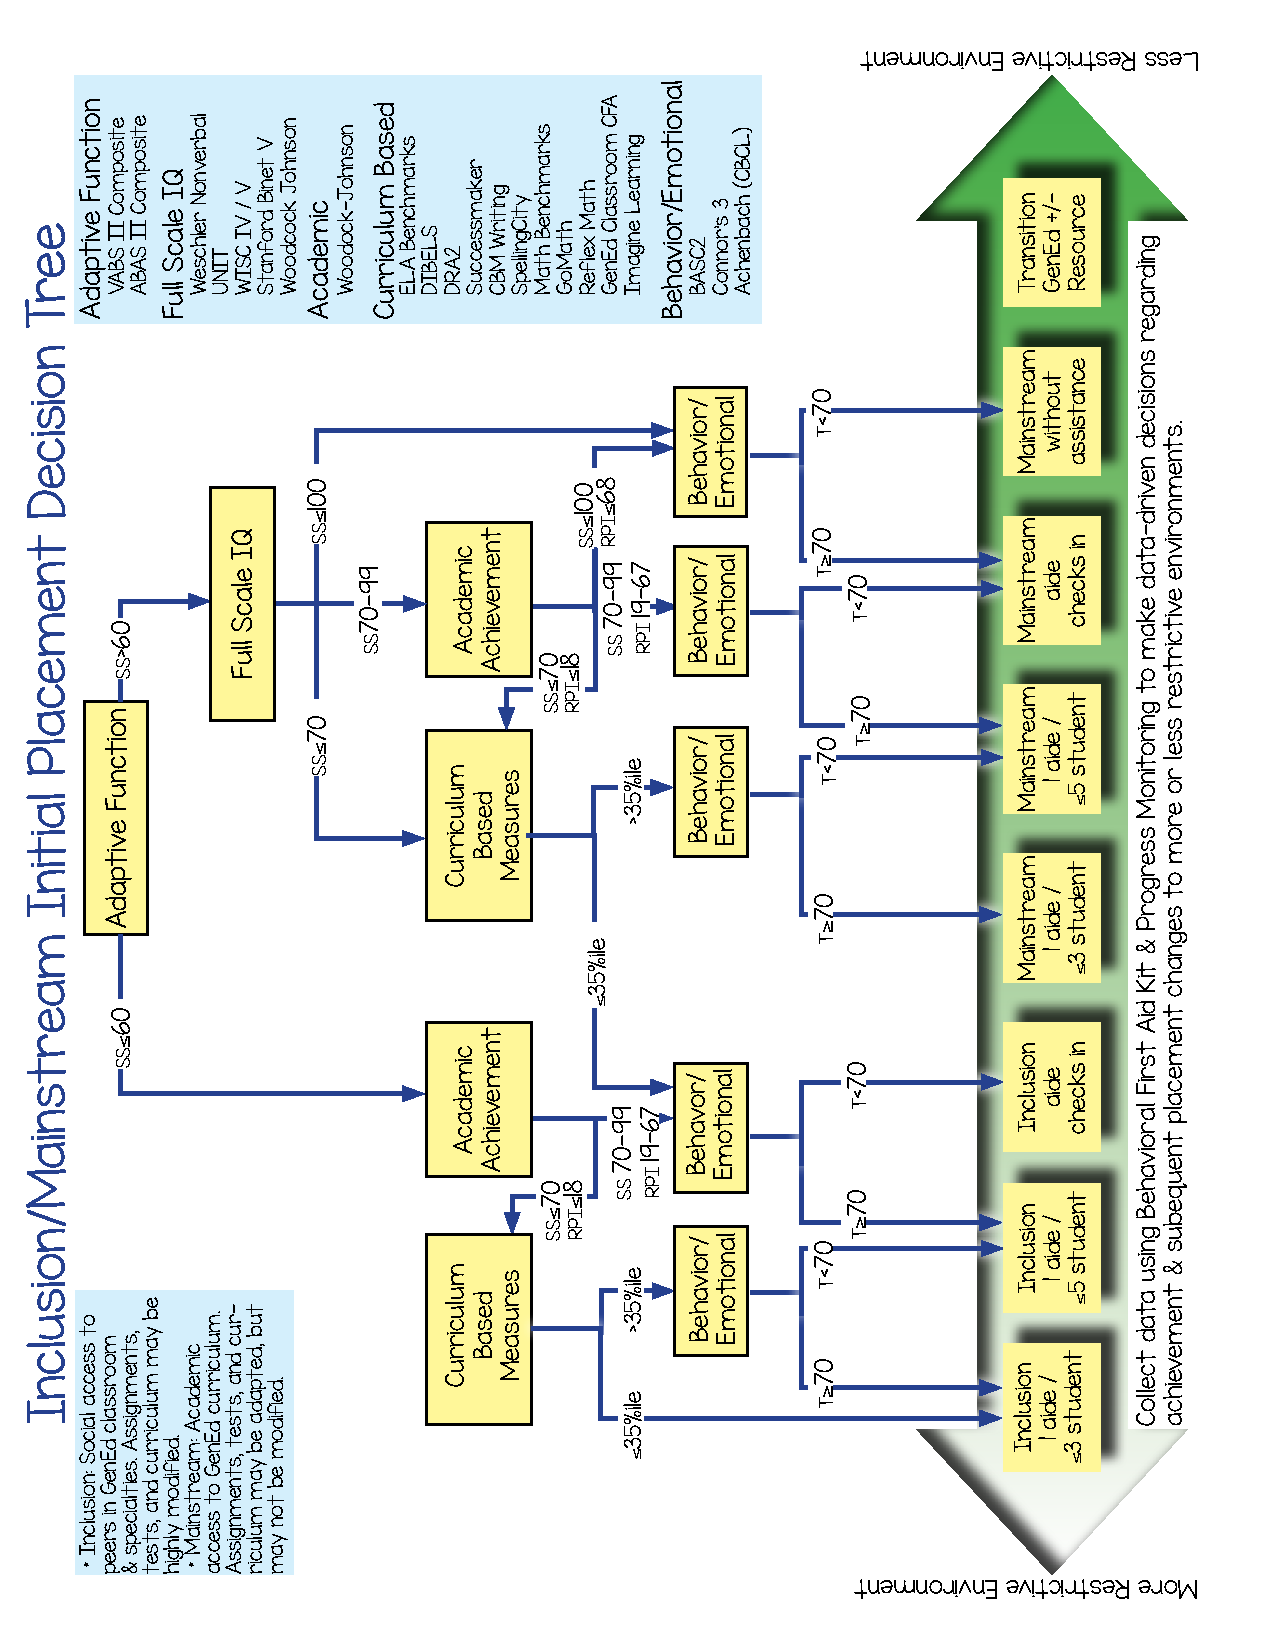
\includepdf[landscape=TRUE, pages={1}]{DecisionTree.pdf}
\label{Appendix2}
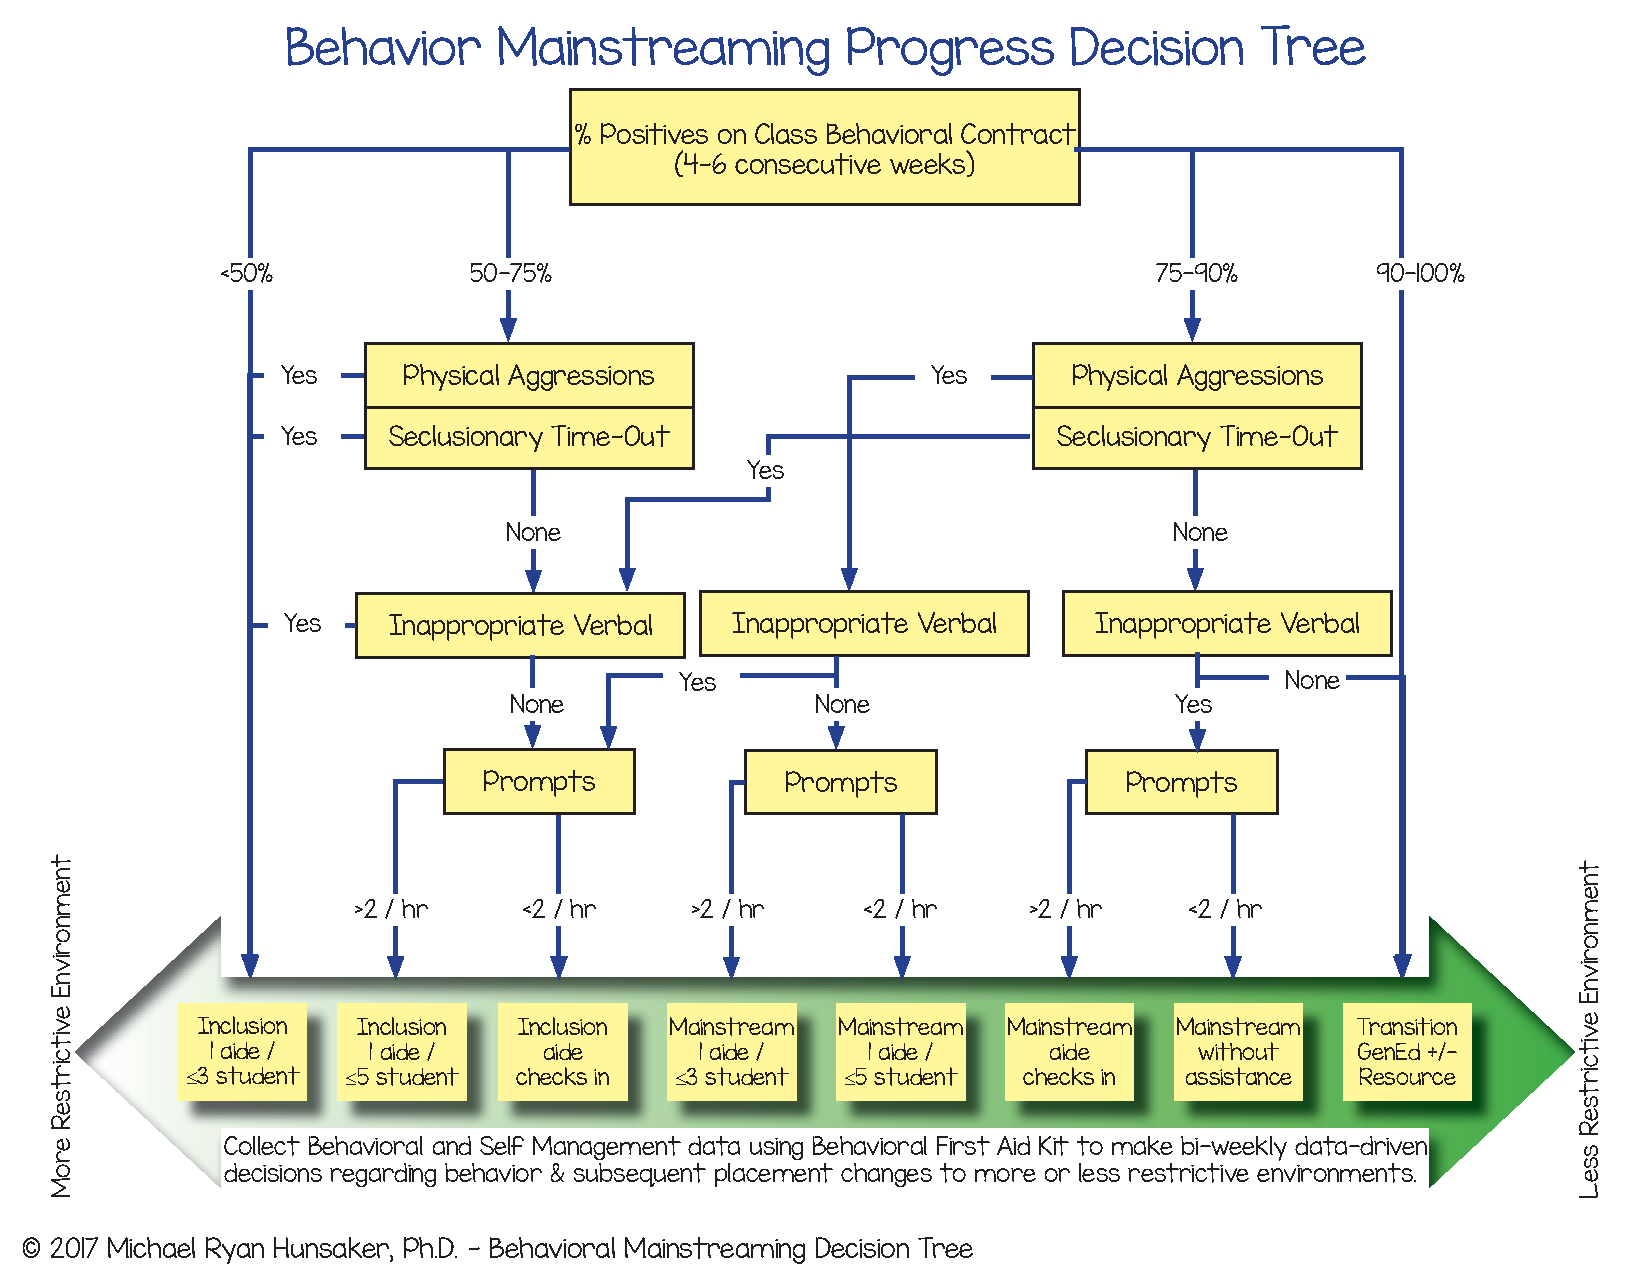
\includepdf[landscape=TRUE, pages={1}]{BehaviorPipeline.pdf}
\label{Appendix3}
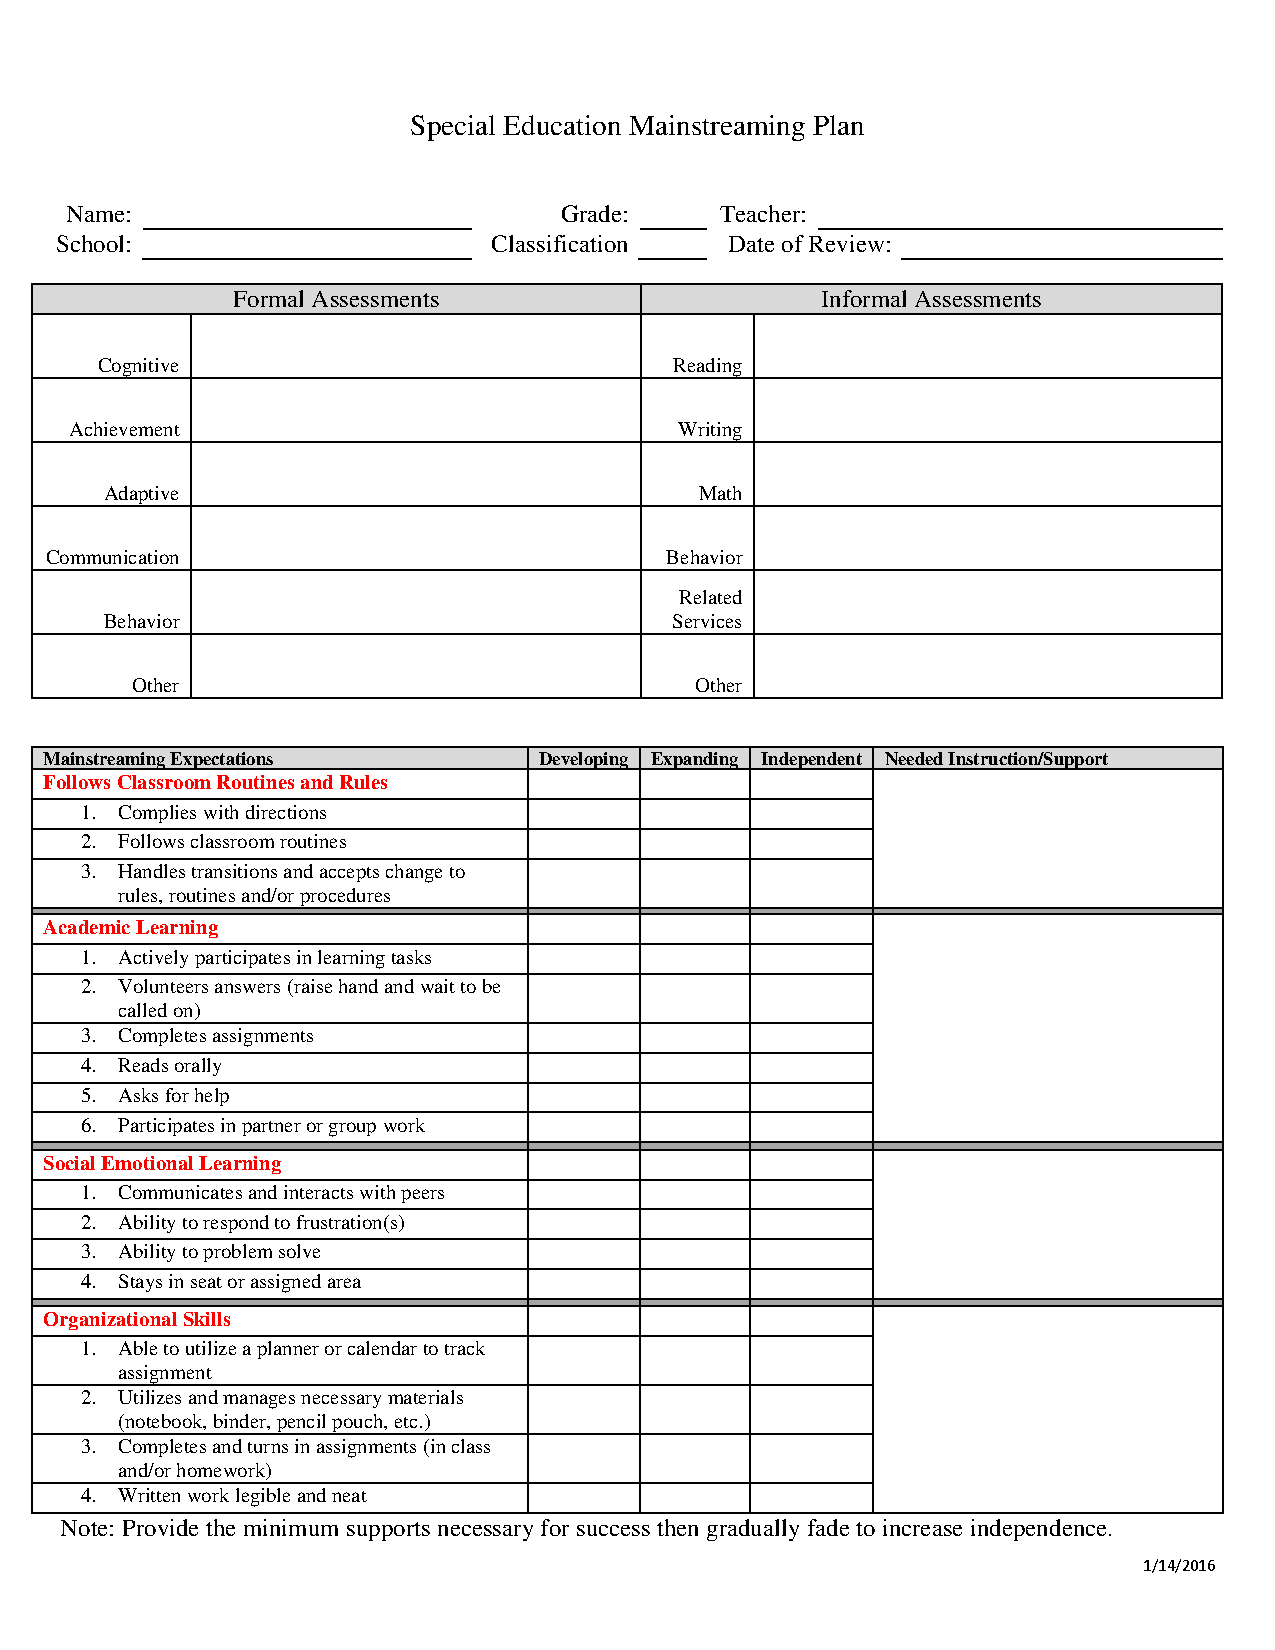
\includepdf[pages={1,2}]{MainstreamingPlan.pdf}
\clearpage \mbox{} \clearpage
\label{Appendix4}
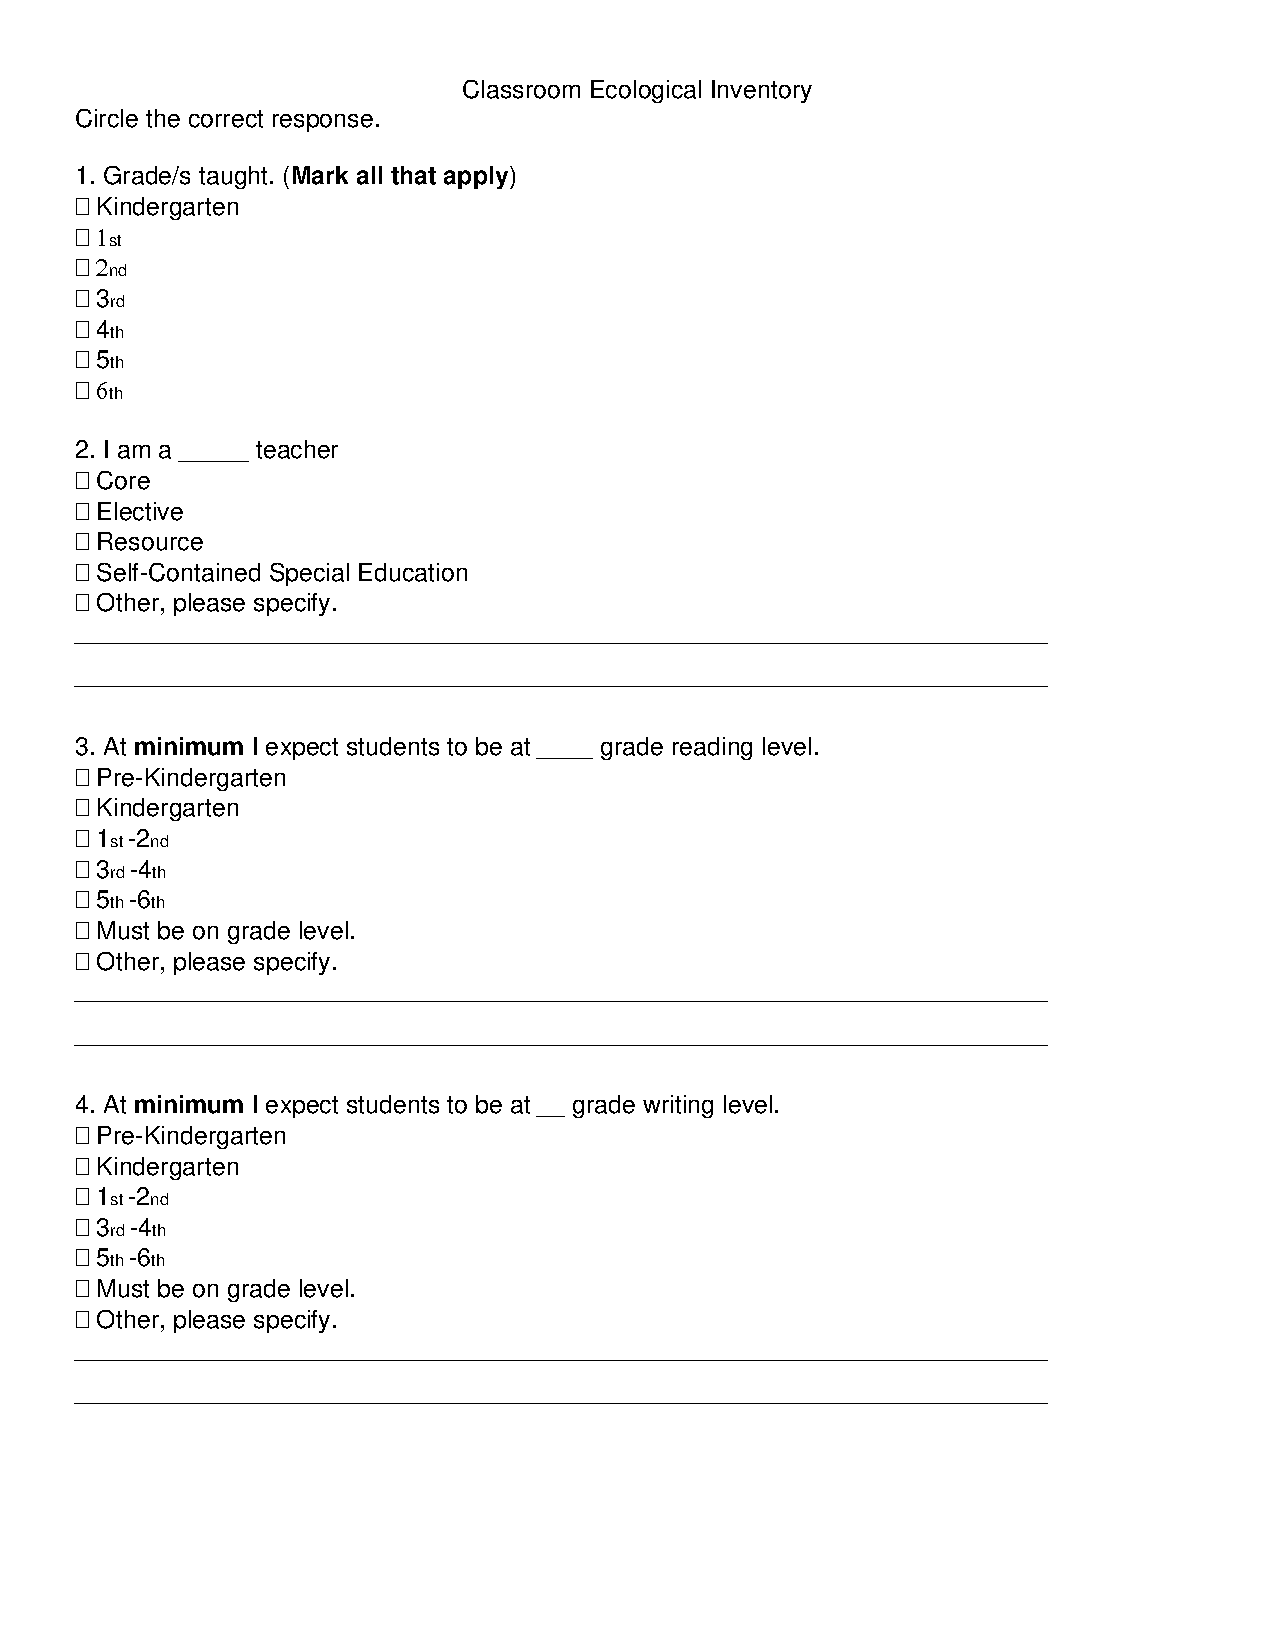
\includepdf[pages={1,2,3,4,5}]{ClassroomEcologicalInventory.pdf}
\clearpage \mbox{} \clearpage
\label{Appendix5}
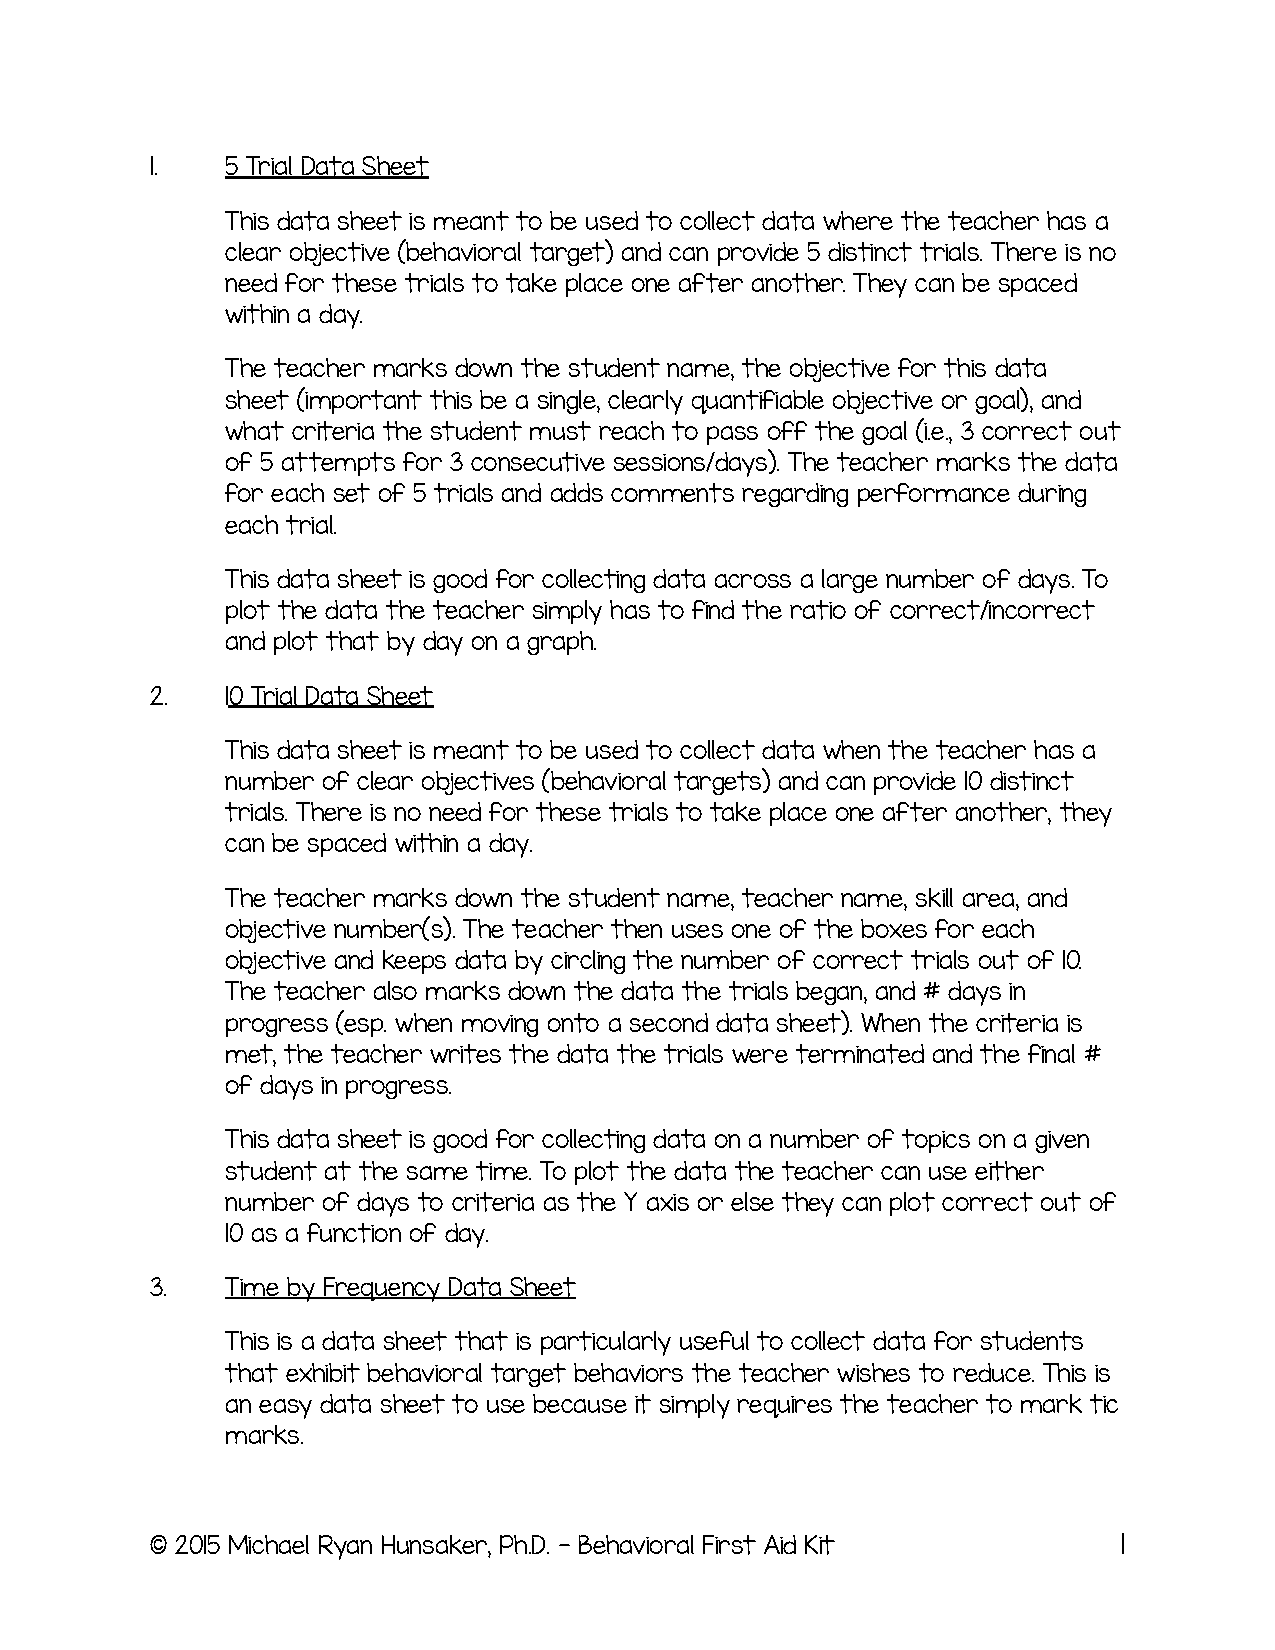
\includepdf[pages={1-56}]{BehavioralFirstAidKit.pdf}
%%%%%%%%%%%%%%%% End Body %%%%%%%%%%%%%%%%%%%%%%%
%
%%%%%%%%%%%% Begin Back Matter %%%%%%%%%%%%%%%%%%%
\addcontentsline{toc}{part}{Notes and Bioliography}
\end{document}